% ============================================================
% PLANTILLA MAESTRA DE GUÍAS — ACADEMIA ZENIT
% Guía de Raíces — Versión 1.1 · 2026
% ============================================================

\documentclass[11pt, letterpaper]{article}

\usepackage[T1]{fontenc}
\usepackage[utf8]{inputenc}
\usepackage[spanish, es-tabla]{babel}
\usepackage[margin=2cm, top=2.2cm, bottom=2.2cm]{geometry}
\usepackage{amsmath, amssymb, amsthm}
\usepackage{mathtools}
\usepackage{array, booktabs, tabularx}
\usepackage{xcolor}
\usepackage{graphicx}
\usepackage{enumitem}
\usepackage{fancyhdr}
\usepackage{tcolorbox}
\usepackage{tikz}
\usetikzlibrary{positioning, babel, arrows.meta}
\usepackage{pgfplots}
\pgfplotsset{compat=1.18}
\usepackage{lastpage}
\usepackage{multicol}
\usepackage{cancel}
\usepackage{calc}
\usepackage{setspace}

% -- Espaciado global --
\linespread{1.18}
\setlength{\parskip}{6pt}
\setlength{\parindent}{0pt}

% -- Espaciado en listas --
\setlist{itemsep=4pt, topsep=6pt, parsep=2pt}
\setlist[enumerate,2]{itemsep=3pt, topsep=3pt}

% -- Colores Institucionales Academia Zenit --
\definecolor{zenitnavy}{HTML}{1A3A5C}
\definecolor{zenitblue}{HTML}{2E6DA4}
\definecolor{zenitgold}{HTML}{C9820A}
\definecolor{zenitlightgray}{HTML}{F5F5F5}
\definecolor{zenitgreen}{HTML}{1A6B3C}
\definecolor{zenitred}{HTML}{8B1A1A}
\definecolor{blocka}{HTML}{1A3A5C}
\definecolor{blockb}{HTML}{1A6B3C}
\definecolor{blockc}{HTML}{7B2D8B}

\tcbuselibrary{skins, breakable}
\tcbset{
  importantbox/.style={enhanced,breakable,colback=white,colframe=zenitblue,
    colbacktitle=zenitblue,coltitle=white,left=10pt,right=10pt,top=12pt,bottom=10pt,
    arc=4pt,leftrule=5pt,fonttitle=\bfseries,
    attach boxed title to top left={xshift=0.5cm,yshift*=-\tcboxedtitleheight/2},
    boxed title style={colframe=zenitblue,colback=zenitblue,arc=2pt}},
  examplebox/.style={enhanced,breakable,colback=white,colframe=zenitgold,
    colbacktitle=zenitgold,coltitle=white,left=10pt,right=10pt,top=12pt,bottom=10pt,
    arc=4pt,leftrule=5pt,fonttitle=\bfseries,
    attach boxed title to top left={xshift=0.5cm,yshift*=-\tcboxedtitleheight/2},
    boxed title style={colframe=zenitgold,colback=zenitgold,arc=2pt}},
  warningbox/.style={enhanced,breakable,colback=white,colframe=zenitred,
    colbacktitle=zenitred,coltitle=white,left=10pt,right=10pt,top=12pt,bottom=10pt,
    arc=4pt,leftrule=5pt,fonttitle=\bfseries,
    attach boxed title to top left={xshift=0.5cm,yshift*=-\tcboxedtitleheight/2},
    boxed title style={colframe=zenitred,colback=zenitred,arc=2pt}},
  answerbox/.style={enhanced,breakable,colback=white,colframe=zenitnavy,
    colbacktitle=zenitnavy,coltitle=white,left=10pt,right=10pt,top=12pt,bottom=10pt,
    arc=4pt,leftrule=5pt,fonttitle=\bfseries,
    attach boxed title to top left={xshift=0.5cm,yshift*=-\tcboxedtitleheight/2},
    boxed title style={colframe=zenitnavy,colback=zenitnavy,arc=2pt}}
}

\newcommand{\seccionheader}[2]{%
  \vspace{1.6em}
  \noindent{\Large\bfseries\color{#1} #2}\par
  \vspace{0.4em}{\noindent\color{#1}\rule{\linewidth}{0.8pt}}
  \vspace{1.0em}}

\newcommand{\subbloque}[1]{%
  \vspace{14pt}
  \noindent{\large\bfseries\color{zenitnavy} #1}\par
  \vspace{4pt}\hrule height 1pt\vspace{8pt}}

\newcommand{\alternativasformato}[3]{%
\item\begin{minipage}[t]{\linewidth}
#1\\
\begin{minipage}{\linewidth}\vspace{7mm}
\begin{tikzpicture}[every node/.style={anchor=north west}]
  \node (texto) at (0,0) {\begin{minipage}{0.58\linewidth}
    \begin{enumerate}[label=\Alph*),leftmargin=14pt]#2\end{enumerate}
    \end{minipage}};
  \node (figura) at (10.4,0) {#3};
\end{tikzpicture}
\end{minipage}\vspace{7mm}
\end{minipage}}

\newcommand{\TipoGuia}{Guía de Estudio Progresiva}
\newcommand{\TituloGuia}{Raíces: construcción continua del concepto}
\newcommand{\TemaEncabezado}{Raíces · 1.1 · 2026}
\newcommand{\NivelGuia}{Matemática}

\pagestyle{fancy}\fancyhf{}
\fancyhead[L]{\small\textbf{Academia Zenit} $\cdot$ \TemaEncabezado}
\fancyhead[R]{\small Página \thepage\ de \pageref{LastPage}}
\fancyfoot[L]{\small\textit{\NivelGuia\ · Raíces}}
\fancyfoot[R]{\small Prohibida su reproducción total o parcial.}

% ============================================================
\begin{document}
% ============================================================
% PORTADA
% ============================================================
\thispagestyle{empty}

\vspace*{2.5cm}

\begin{center}
  
\includegraphics[width=0.30\linewidth]{logosin fondo.png}\\[1.8cm]
  {\Huge\bfseries\color{zenitnavy} ACADEMIA ZENIT}\\[0.5cm]
  {\LARGE\bfseries\color{zenitblue} Guía de Estudio Progresiva}\\[0.3cm]
  {\LARGE\bfseries\color{zenitblue} Raíces: construcción continua del concepto}\\[1.4cm]
  {\Large\bfseries\color{zenitnavy} Matemática}\\[1.2cm]
  \textcolor{zenitnavy}{\rule{0.72\linewidth}{1.5pt}}\\[1.0cm]
  {\large\itshape\color{zenitnavy} Material de apoyo y ejercitación}
\end{center}

\vfill

\begin{center}
  \textcolor{zenitnavy}{\rule{0.72\linewidth}{0.6pt}}\\[0.5cm]
  {\large\bfseries\color{zenitnavy} Academia Zenit}\\[3pt]
  {\color{zenitgold} Matemática · Raíces · 1.1 · 2026}\\[0.4cm]
  \textcolor{zenitnavy}{\rule{0.72\linewidth}{0.6pt}}
\end{center}

% ============================================================
% PÁGINA 2 — GLOSARIO E ÍNDICE
% ============================================================
\clearpage
\thispagestyle{empty}

\vspace*{0.2cm}

% ---- GLOSARIO ----

\begin{tcolorbox}[importantbox, title={Glosario de simbología}]

{\small\textit{Los símbolos específicos del tema raíces aparecen resaltados en \textcolor{zenitgold}{\textbf{dorado}}.}}

\medskip
\begin{center}
\renewcommand{\arraystretch}{1.32}
\begin{tabular}{c p{4.8cm} | c p{4.8cm}}
\toprule
\textbf{Símbolo} & \textbf{Significado} & \textbf{Símbolo} & \textbf{Significado}\\
\midrule
\multicolumn{4}{l}{\textit{Conjuntos numéricos}}\\
$\mathbb{N}$ & Naturales $\{1,2,3,\ldots\}$ &
$\mathbb{Z}$ & Enteros $\{\ldots,-1,0,1,\ldots\}$\\
$\mathbb{Q}$ & Racionales $\frac{p}{q}$, $q\neq 0$ &
$\mathbb{R}$ & Números reales\\
$a \in A$ & $a$ pertenece al conjunto $A$ &
$\{a,b,c\}$ & Conjunto de elementos\\[3pt]
\multicolumn{4}{l}{\textit{Relaciones y lógica}}\\
$=\ \neq$ & Igual / distinto de &
$<\ >\ \leq\ \geq$ & Menor, mayor (estricto y no estricto)\\
$\approx$ & Aproximadamente igual &
$|a|$ & Valor absoluto de $a$\\
$\Rightarrow$ & Implica (consecuencia) &
$\Leftrightarrow$ & Si y solo si (equivalencia)\\[3pt]
\multicolumn{4}{l}{\textit{Aritmética y álgebra}}\\
$a^n$ & $a$ elevado a la potencia $n$ &
$\dfrac{p}{q}$ & Fracción entre $p$ y $q$\\
$\text{m.c.m.}(a,b)$ & Mínimo común múltiplo &
$\text{m.c.d.}(a,b)$ & Máximo común divisor\\[3pt]
\multicolumn{4}{l}{\textit{\textcolor{zenitgold}{\textbf{Raíces y potencias racionales — tema central}}}}\\
\textcolor{zenitgold}{$\sqrt{a}$} & \textcolor{zenitgold}{Raíz cuadrada de $a$} &
\textcolor{zenitgold}{$\sqrt[n]{a}$} & \textcolor{zenitgold}{Raíz enésima de $a$; $n$: índice}\\
\textcolor{zenitgold}{$\sqrt[3]{a}$} & \textcolor{zenitgold}{Raíz cúbica de $a$} &
\textcolor{zenitgold}{$a^{m/n}$} & \textcolor{zenitgold}{Potencia de exponente racional}\\
\textcolor{zenitgold}{$a\sqrt[n]{b}$} & \textcolor{zenitgold}{Coeficiente $a$ · raíz $\sqrt[n]{b}$} &
\textcolor{zenitgold}{$\sqrt[n]{a^m}$} & \textcolor{zenitgold}{Raíz de potencia: equivale a $a^{m/n}$}\\
\textcolor{zenitgold}{$\sqrt[n]{\sqrt[m]{a}}$} & \textcolor{zenitgold}{Raíz de raíz $= \sqrt[nm]{a}$} &
\textcolor{zenitgold}{$\sqrt{a}\pm\sqrt{b}$} & \textcolor{zenitgold}{Binomio con raíces}\\[3pt]
\multicolumn{4}{l}{\textit{Convenciones de esta guía}}\\
$\checkmark$ & Solución verificada en la original &
$\times$ & Solución extraña: se descarta\\
$\bigstar$ & Nivel básico &
$\bigstar\bigstar\bigstar$ & Nivel avanzado\\
\bottomrule
\end{tabular}
\end{center}
\end{tcolorbox}

\medskip

% ---- ÍNDICE ----

\begin{tcolorbox}[answerbox, title={Índice de contenidos}]
\begin{multicols}{2}
{\small
\begin{tabular}{r @{\hspace{4pt}} p{5.5cm} @{\hspace{6pt}} r}
\textbf{\S{}} & \textbf{Galería matemática} & \textbf{p.\,\pageref{sec:galeria}}\\
 & Hipatia de Alejandría & \\
 & Al-Juarismi & \\[3pt]
\textbf{\S{}} & \textbf{Sección 1 · Raíz cuadrada} & \textbf{p.\,\pageref{sec:1}}\\
1.1 & La pregunta que da origen al concepto & \pageref{sub:1.1}\\
1.2 & Cuadrados perfectos & \pageref{sub:1.2}\\
1.3 & Números irracionales & \pageref{sub:1.3}\\
1.4 & Propiedad de orden & \pageref{sub:1.4}\\
1.5 & Dos estrategias para ordenar & \pageref{sub:1.5}\\
1.6 & Estimación por aproximación & \pageref{sub:1.6}\\[3pt]
\textbf{\S{}} & \textbf{Sección 2 · Raíz cúbica y enésima} & \textbf{p.\,\pageref{sec:2}}\\
2.1 & La raíz cúbica: volumen y arista & \pageref{sub:2.1}\\
2.2 & La raíz enésima: generalización & \pageref{sub:2.2}\\[3pt]
\textbf{\S{}} & \textbf{Sección 3 · Propiedades} & \textbf{p.\,\pageref{sec:3}}\\
3.1 & Relación inversa & \pageref{sub:3.1}\\
3.2 & Propiedades P1 y P2 & \pageref{sub:3.2}\\
3.3 & Simplificación de raíces & \pageref{sub:3.3}\\
3.4 & Suma y resta de semejantes & \pageref{sub:3.4}\\
\end{tabular}

\columnbreak

\begin{tabular}{r @{\hspace{4pt}} p{5.5cm} @{\hspace{6pt}} r}
\textbf{\S{}} & \textbf{Sección 4 · Multiplicación} & \textbf{p.\,\pageref{sec:4}}\\
4.1 & Mismo índice & \pageref{sub:4.1}\\
4.2 & Distinto índice (m.c.m.) & \pageref{sub:4.2}\\
4.3 & Productos notables & \pageref{sub:4.3}\\[3pt]
\textbf{\S{}} & \textbf{Sección 5 · Potencias racionales} & \textbf{p.\,\pageref{sec:5}}\\
5.1 & Motivación y equivalencia & \pageref{sub:5.1}\\
5.2 & Propiedades & \pageref{sub:5.2}\\
5.3 & Cambio de índice & \pageref{sub:5.3}\\
5.4 & Raíz de una raíz y raíz única & \pageref{sub:5.4}\\[3pt]
\textbf{\S{}} & \textbf{Sección 6 · Racionalización} & \textbf{p.\,\pageref{sec:6}}\\
6.2 & Caso 1: denominador $\sqrt{a}$ & \pageref{sub:6.2}\\
6.3 & Caso 2: denominador $\sqrt[n]{a^k}$ & \pageref{sub:6.3}\\
6.4 & Caso 3: conjugado & \pageref{sub:6.4}\\
6.5 & Caso 4: raíces cúbicas & \pageref{sub:6.5}\\
6.6 & Caso 5: trinomios y anidadas & \pageref{sub:6.6}\\[3pt]
\textbf{\S{}} & \textbf{Sección 7 · Ecuaciones y geometría} & \textbf{p.\,\pageref{sec:7}}\\
 & Ejercicios con alternativas & \pageref{sub:ej.alt}\\
 & Ejercicios de desarrollo & \pageref{sub:ej.des}\\[3pt]
\textbf{\S{}} & \textbf{Ejercicios tipo PAES} & \textbf{p.\,\pageref{sec:paes}}\\[3pt]
\textbf{\S{}} & \textbf{Solucionario completo} & \textbf{p.\,\pageref{sec:sol}}\\
\end{tabular}
}
\end{multicols}
\end{tcolorbox}

\medskip

% ---- PROPÓSITO ----

\begin{tcolorbox}[importantbox, title={Propósito de la guía}]
Esta guía construye el concepto de \textbf{raíz} de forma continua y rigurosamente progresiva: cada sección usa únicamente herramientas ya introducidas en secciones anteriores. El recorrido parte de la raíz cuadrada como idea geométrica concreta y llega hasta la operatoria completa con potencias racionales, racionalización y ecuaciones con raíces.

\smallskip
\textbf{Dificultad:} $\bigstar$ básico \quad $\bigstar\bigstar$ intermedio \quad $\bigstar\bigstar\bigstar$ avanzado. \quad \textbf{Notación:} $\sqrt[2]{a}=\sqrt{a}$; sin índice escrito, el índice es siempre 2.
\end{tcolorbox}

% ============================================================
% PÁGINA 4 — GALERÍA MATEMÁTICA
% ============================================================
\clearpage
\thispagestyle{empty}
\label{sec:galeria}

\begin{center}
  \vspace*{0.4cm}
  \textcolor{zenitnavy}{\rule{0.72\linewidth}{1.2pt}}\\[0.5cm]
  {\Large\bfseries\color{zenitnavy} Galería matemática}\\[0.15cm]
  {\normalsize\itshape\color{zenitgold} Quienes construyeron las herramientas que usamos hoy}\\[0.4cm]
  \textcolor{zenitnavy}{\rule{0.72\linewidth}{0.6pt}}
\end{center}

\vspace{0.6cm}

% ---- HIPATIA ----

\begin{tcolorbox}[enhanced, breakable,
  colback=white, colframe=blockb, colbacktitle=blockb,
  coltitle=white, arc=4pt, leftrule=5pt,
  left=10pt, right=10pt, top=12pt, bottom=10pt,
  fonttitle=\bfseries,
  attach boxed title to top left={xshift=0.5cm, yshift*=-\tcboxedtitleheight/2},
  boxed title style={colframe=blockb, colback=blockb, arc=2pt},
  title={Hipatia de Alejandría \hfill \normalfont\itshape c.\,360 — 415 d.C.}]

\begin{minipage}[t]{0.18\linewidth}
\vspace{0pt}
% -------------------------------------------------------
% RETRATO: reemplazar el bloque tikzpicture por:
%   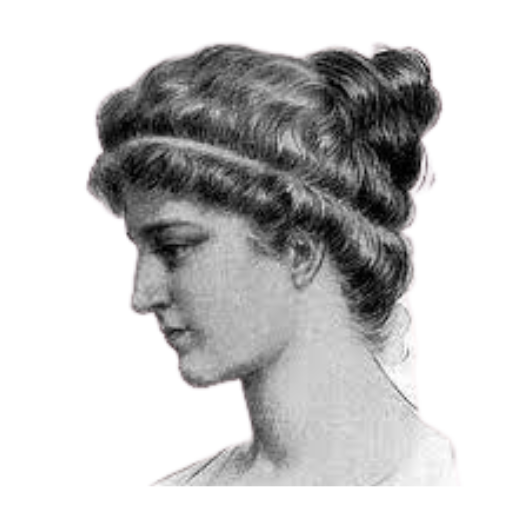
\includegraphics[width=\linewidth, height=3.2cm,
%     keepaspectratio]{hipatia.jpg}
% El archivo debe estar en la misma carpeta que el .tex
% Nombre sugerido: hipatia.jpg  (o .png)
% -------------------------------------------------------
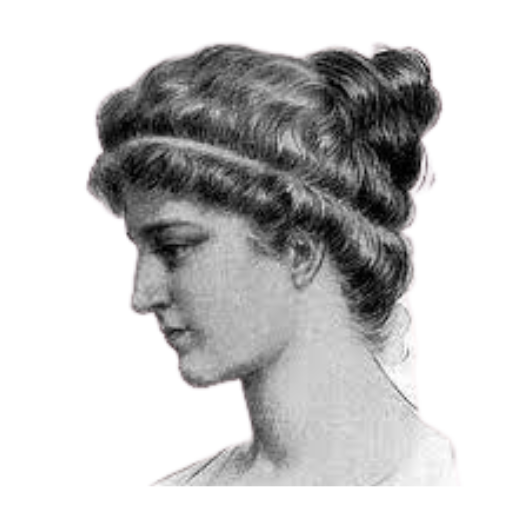
\includegraphics[width=\linewidth, height=3.2cm, keepaspectratio]{hipatia.png}
\end{minipage}
\hfill
\begin{minipage}[t]{0.78\linewidth}
\vspace{0pt}

Hipatia fue la \textbf{primera matemática de cuya vida y obra tenemos registro histórico documentado}. Nacida en Alejandría, ciudad que entonces era el centro intelectual del mundo mediterráneo, aprendió matemáticas y filosofía de su padre Teón, último miembro documentado del \textit{Mouseion} alejandrino y autor de importantes comentarios sobre Euclides y Ptolomeo.

\medskip
Fue directora de la escuela neoplatónica de Alejandría, y sus clases atraían estudiantes de todo el Imperio Romano. Escribió comentarios sobre la \textit{Aritmética} de Diofanto —obra central de la teoría de números y las ecuaciones algebraicas— y sobre las \textit{Cónicas} de Apolonio. Aunque ninguna de sus obras sobrevivió, las cartas de su discípulo Sinesio de Cirene atestiguan un pensamiento riguroso y una pedagogía excepcional.

\medskip
\textbf{Conexión con este tema:} las \textit{Cónicas} que Hipatia comentó describen figuras geométricas —parábolas, elipses, hipérbolas— cuyas medidas fundamentales como distancias y semiejes involucran directamente raíces cuadradas. Su trabajo contribuyó a que esas herramientas geométricas se mantuvieran vivas en la tradición matemática.
\end{minipage}

\end{tcolorbox}

\vspace{0.7cm}

% ---- AL-JUARISMI ----

\begin{tcolorbox}[enhanced, breakable,
  colback=white, colframe=blockc, colbacktitle=blockc,
  coltitle=white, arc=4pt, leftrule=5pt,
  left=10pt, right=10pt, top=12pt, bottom=10pt,
  fonttitle=\bfseries,
  attach boxed title to top left={xshift=0.5cm, yshift*=-\tcboxedtitleheight/2},
  boxed title style={colframe=blockc, colback=blockc, arc=2pt},
  title={Muhammad ibn M\={u}s\={a} al-Juarismi \hfill \normalfont\itshape c.\,780 — 850 d.C.}]

\begin{minipage}[t]{0.78\linewidth}
\vspace{0pt}

Al-Juarismi fue matemático, astrónomo y geógrafo en la \textit{Bayt al-Hikma} (Casa de la Sabiduría) de Bagdad bajo el califato de al-Ma'mun. Su tratado \textit{Al-Kitab al-mukhtasar fi hisab al-jabr wal-muqabala} («Compendio sobre el cálculo por reintegración y equiparación», c.\,820) es \textbf{el documento fundacional del álgebra como disciplina independiente} y el primer texto que sistematiza la resolución de ecuaciones de primer y segundo grado de manera elemental y para uso práctico.

\medskip
El título de ese tratado dio origen a la palabra \textit{álgebra} (de \textit{al-jabr}, «restauración»). Y el nombre latinizado de su autor —\textit{Algoritmi}— dio origen a la palabra \textbf{algoritmo}, que hoy designa cualquier procedimiento paso a paso para resolver un problema.

\medskip
\textbf{Conexión directa con este tema:} al-Juarismi necesitaba las raíces cuadradas para resolver ecuaciones de segundo grado. En su tratado aparecen procedimientos geométricos y algebraicos para calcular $\sqrt{n}$ y expresar soluciones del tipo $x = \sqrt{a} + b$, demostrando la completación del cuadrado con justificaciones geométricas. Fue el primero en tratar las raíces como resultados legítimos y manipulables dentro del álgebra.
\end{minipage}
\hfill
\begin{minipage}[t]{0.18\linewidth}
\vspace{0pt}
% -------------------------------------------------------
% RETRATO: reemplazar el bloque tikzpicture por:
%   \includegraphics[width=\linewidth, height=3.2cm,
%     keepaspectratio]{aljuarismi.jpg}
% El archivo debe estar en la misma carpeta que el .tex
% Nombre sugerido: aljuarismi.jpg  (o .png)
% -------------------------------------------------------
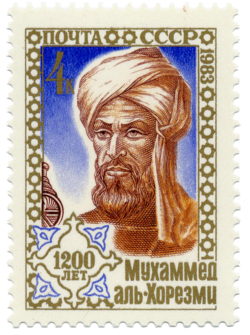
\includegraphics[width=\linewidth, height=3.2cm, keepaspectratio]{al-juarismi.png}
\end{minipage}

\end{tcolorbox}

\vspace{0.5cm}
\begin{center}
  \textcolor{zenitgold}{\rule{0.5\linewidth}{0.5pt}}\\[0.3cm]
  {\small\itshape\color{zenitnavy} La matemática no tiene fronteras de época, género ni cultura.}\\[0.2cm]
  \textcolor{zenitgold}{\rule{0.5\linewidth}{0.5pt}}
\end{center}

\clearpage
\thispagestyle{empty}
\phantom{x}
\clearpage

% ============================================================
% SECCIÓN 1
% ============================================================
\clearpage
\seccionheader{blocka}{Sección 1 · La raíz cuadrada: del cuadrado al número}
\label{sec:1}

\subbloque{1.1 La pregunta que da origen al concepto}
\label{sub:1.1}

Si conocemos el \textbf{área} de un cuadrado, ¿podemos calcular cuánto mide su lado? La respuesta a esa pregunta es la raíz cuadrada.

\begin{center}
\begin{tikzpicture}[scale=0.44]
  \draw[fill=zenitlightgray,draw=zenitnavy,very thick](0,0)rectangle(1,1);
  \node[below]at(0.5,-0.15){\small$A=1$};\node[below]at(0.5,-0.75){\small lado$=1$};
  \draw[fill=zenitlightgray,draw=zenitnavy,very thick](3,0)rectangle(5,2);
  \node[below]at(4,-0.15){\small$A=4$};\node[below]at(4,-0.75){\small lado$=2$};
  \draw[fill=zenitlightgray,draw=zenitnavy,very thick](7,0)rectangle(10,3);
  \node[below]at(8.5,-0.15){\small$A=9$};\node[below]at(8.5,-0.75){\small lado$=3$};
  \draw[fill=zenitlightgray,draw=zenitnavy,very thick](12,0)rectangle(16,4);
  \node[below]at(14,-0.15){\small$A=16$};\node[below]at(14,-0.75){\small lado$=4$};
  \draw[fill=zenitlightgray,draw=zenitnavy,very thick](18,0)rectangle(23,5);
  \node[below]at(20.5,-0.15){\small$A=25$};\node[below]at(20.5,-0.75){\small lado$=5$};
\end{tikzpicture}
\end{center}

\begin{tcolorbox}[importantbox, title={Definición formal — Raíz cuadrada}]
La \textbf{raíz cuadrada} de un número $a \geq 0$, escrita $\sqrt{a}$, es el único número \emph{no negativo} $b$ tal que $b^2 = a$:
$$\sqrt{a} = b \quad\Longleftrightarrow\quad b^2 = a, \quad b \geq 0$$

Al símbolo $\sqrt{\phantom{a}}$ se le llama \textbf{radical}; al número bajo el radical, \textbf{radicando}; el 2 es el \textbf{índice} y no se escribe.

La raíz cuadrada de $a$ \textbf{solo existe en los reales cuando $a \geq 0$}. Si $a < 0$, no hay ningún número real cuyo cuadrado sea $a$.
\end{tcolorbox}

\begin{tcolorbox}[warningbox, title={Error frecuente — el signo de la raíz}]
$\sqrt{49}=7$, \textbf{nunca} $-7$ ni $\pm 7$. La raíz cuadrada entrega siempre el valor positivo. Lo que sí se puede escribir es $-\sqrt{49}=-7$ para referirse a la raíz negativa. El símbolo $\pm$ aparece \emph{solo} al resolver ecuaciones: $x^2=49 \Rightarrow x=\pm 7$. Pero $\sqrt{49}$ es uno solo: $7$.
\end{tcolorbox}

\begin{tcolorbox}[examplebox, title={Ejemplos — definición y existencia}]
\begin{enumerate}[label=\textbf{Ej. \arabic*.}, leftmargin=*, itemsep=12pt]

\item \textbf{¿Cuánto mide el lado de un cuadrado de área 36 cm$^2$?}

Buscamos $b$ tal que $b^2 = 36$. Como $6^2 = 36$, el lado mide $\sqrt{36} = 6$ cm.

\textbf{Verificación:} $6^2 = 36$. \checkmark \quad \textbf{Conclusión:} el lado mide $6$ cm.

\item \textbf{¿Existe un cuadrado de área $-4$ cm$^2$?}

No, porque el área es siempre positiva. Matemáticamente, $\sqrt{-4}$ no existe en $\mathbb{R}$: ningún número real elevado al cuadrado da $-4$.

\end{enumerate}
\end{tcolorbox}

\medskip
\textbf{Practica inmediata} \quad $\bigstar$ — ¿Cuánto mide el lado del cuadrado con el área indicada? Si la raíz no existe, explica por qué:
\begin{multicols}{4}
\begin{enumerate}[label=\alph*), leftmargin=*]
  \item $A = 4$ cm$^2$
  \item $A = 25$ cm$^2$
  \item $A = 64$ cm$^2$
  \item $A = 100$ cm$^2$
  \item $A = -9$ cm$^2$
  \item $A = 0$ cm$^2$
  \item $A = 1$ cm$^2$
  \item $A = 49$ cm$^2$
\end{enumerate}
\end{multicols}

\subbloque{1.2 Cuadrados perfectos: cuando la raíz es exacta}
\label{sub:1.2}

Un número natural es un \textbf{cuadrado perfecto} si su raíz cuadrada también es un número natural. Solo en estos casos la raíz es exacta.

\begin{tcolorbox}[importantbox, title={Tabla de cuadrados perfectos — del 1 al 20}]
\begin{center}
\renewcommand{\arraystretch}{1.3}
\begin{tabular}{c|c|c||c|c|c}
\toprule
$n$ & $n^2$ & $\sqrt{n^2}$ & $n$ & $n^2$ & $\sqrt{n^2}$\\
\midrule
1  & 1   & 1  & 11 & 121 & 11\\
2  & 4   & 2  & 12 & 144 & 12\\
3  & 9   & 3  & 13 & 169 & 13\\
4  & 16  & 4  & 14 & 196 & 14\\
5  & 25  & 5  & 15 & 225 & 15\\
6  & 36  & 6  & 16 & 256 & 16\\
7  & 49  & 7  & 17 & 289 & 17\\
8  & 64  & 8  & 18 & 324 & 18\\
9  & 81  & 9  & 19 & 361 & 19\\
10 & 100 & 10 & 20 & 400 & 20\\
\bottomrule
\end{tabular}
\end{center}
Memorizar esta tabla permite calcular raíces exactas de forma inmediata y es la base de toda la sección.
\end{tcolorbox}

\begin{tcolorbox}[examplebox, title={Ejemplos — cuadrados perfectos}]
\begin{enumerate}[label=\textbf{Ej. \arabic*.}, leftmargin=*, itemsep=12pt]

\item \textbf{Calcular $\sqrt{49}$, $\sqrt{169}$ y $\sqrt{400}$}

Buscamos en la tabla el entero cuyo cuadrado coincide con el radicando:
\begin{itemize}[itemsep=3pt]
  \item $\sqrt{49}=7$, pues $7^2=49$. \hfill\checkmark
  \item $\sqrt{169}=13$, pues $13^2=169$. \hfill\checkmark
  \item $\sqrt{400}=20$, pues $20^2=400$. \hfill\checkmark
\end{itemize}

\item \textbf{¿Es 50 un cuadrado perfecto?}

Buscamos en la tabla: $7^2=49$ y $8^2=64$. Como $49 < 50 < 64$, no existe ningún entero cuyo cuadrado sea exactamente 50.

\textbf{Conclusión:} 50 \textbf{no} es un cuadrado perfecto; $\sqrt{50}$ no tiene valor exacto entero.

\end{enumerate}
\end{tcolorbox}

\medskip
\textbf{Practica inmediata} \quad $\bigstar$ — Calcula directamente con la tabla:
\begin{multicols}{5}
\begin{enumerate}[label=\alph*), leftmargin=*]
  \item $\sqrt{1}$
  \item $\sqrt{36}$
  \item $\sqrt{81}$
  \item $\sqrt{144}$
  \item $\sqrt{225}$
  \item $\sqrt{4}$
  \item $\sqrt{100}$
  \item $\sqrt{169}$
  \item $\sqrt{289}$
  \item $\sqrt{400}$
\end{enumerate}
\end{multicols}

\subbloque{1.3 Números irracionales: cuando la raíz no es exacta}
\label{sub:1.3}

Si el radicando no es un cuadrado perfecto, su raíz no puede escribirse como número entero ni como fracción. Estos números se llaman \textbf{irracionales}.

\begin{tcolorbox}[importantbox, title={Números racionales e irracionales}]
\begin{itemize}
  \item Un número es \textbf{racional} si puede escribirse como $\dfrac{p}{q}$ con $p,q\in\mathbb{Z}$, $q\neq 0$. Su expansión decimal es finita o periódica. Ejemplos: $3$, $\tfrac{1}{2}$, $0{,}\overline{3}$.
  \item Un número es \textbf{irracional} si \emph{no} puede escribirse así. Su expansión decimal es infinita y sin período. Ejemplos: $\sqrt{2}=1{,}41421\ldots$, $\pi$, $e$.
\end{itemize}

\textbf{Regla práctica:} $\sqrt{n}$ es irracional si y solo si $n$ \textbf{no} es un cuadrado perfecto.
\end{tcolorbox}

\begin{tcolorbox}[examplebox, title={Ejemplos — clasificar como racional o irracional}]
\begin{enumerate}[label=\textbf{Ej. \arabic*.}, leftmargin=*, itemsep=12pt]

\item \textbf{Clasificar: $\sqrt{16}$, $\sqrt{7}$, $\sqrt{225}$, $\sqrt{50}$}

Aplicamos la regla: $\sqrt{n}$ es racional si y solo si $n$ es cuadrado perfecto.
\begin{itemize}[itemsep=3pt]
  \item $\sqrt{16}$: como $4^2=16$, tenemos $\sqrt{16}=4$. \textbf{Racional.}
  \item $\sqrt{7}$: $2^2=4$ y $3^2=9$; 7 no es cuadrado perfecto. \textbf{Irracional.}
  \item $\sqrt{225}$: como $15^2=225$, tenemos $\sqrt{225}=15$. \textbf{Racional.}
  \item $\sqrt{50}$: $7^2=49$ y $8^2=64$; 50 no es cuadrado perfecto. \textbf{Irracional.}
\end{itemize}

\end{enumerate}
\end{tcolorbox}

\medskip
\textbf{Practica inmediata} \quad $\bigstar$ — Clasifica como racional o irracional. Si es racional, escribe su valor:
\begin{multicols}{4}
\begin{enumerate}[label=\alph*), leftmargin=*]
  \item $\sqrt{4}$
  \item $\sqrt{5}$
  \item $\sqrt{121}$
  \item $\sqrt{50}$
  \item $\sqrt{196}$
  \item $\sqrt{200}$
  \item $\sqrt{324}$
  \item $\sqrt{300}$
\end{enumerate}
\end{multicols}

\subbloque{1.4 Propiedad de orden: comparar sin calcular decimales}
\label{sub:1.4}

\begin{tcolorbox}[importantbox, title={Propiedad de orden — las raíces preservan el orden de los radicandos}]
Para $a \geq 0$ y $b \geq 0$:
$$a < b \quad\Longleftrightarrow\quad \sqrt{a} < \sqrt{b}$$

Para comparar $\sqrt{a}$ con $\sqrt{b}$, basta comparar $a$ con $b$, sin calcular nada.

Para comparar $\sqrt{a}$ con un entero $k$, basta comparar $a$ con $k^2$:
$$\sqrt{a} < k \;\Leftrightarrow\; a < k^2 \qquad\text{y}\qquad \sqrt{a} > k \;\Leftrightarrow\; a > k^2$$
\end{tcolorbox}

\begin{tcolorbox}[examplebox, title={Ejemplos — comparar con la propiedad de orden}]
\begin{enumerate}[label=\textbf{Ej. \arabic*.}, leftmargin=*, itemsep=12pt]

\item \textbf{Comparar $\sqrt{50}$ con $7$, sin calcular decimales}

Escribimos $7 = \sqrt{49}$. Como $50 > 49$:
$$\sqrt{50} > \sqrt{49} = 7$$
\textbf{Conclusión:} $\sqrt{50} > 7$.

\item \textbf{Comparar $\sqrt{75}$ con $9$, sin calcular decimales}

Escribimos $9 = \sqrt{81}$. Como $75 < 81$:
$$\sqrt{75} < \sqrt{81} = 9$$
\textbf{Conclusión:} $\sqrt{75} < 9$.

\end{enumerate}
\end{tcolorbox}

\medskip
\textbf{Practica inmediata} \quad $\bigstar$ — Compara sin calcular decimales. Indica $<$, $>$ o $=$:
\begin{multicols}{3}
\begin{enumerate}[label=\alph*), leftmargin=*]
  \item $\sqrt{20}$ \quad vs \quad $4$
  \item $\sqrt{35}$ \quad vs \quad $6$
  \item $\sqrt{100}$ \quad vs \quad $10$
  \item $\sqrt{48}$ \quad vs \quad $7$
  \item $\sqrt{120}$ \quad vs \quad $11$
  \item $\sqrt{63}$ \quad vs \quad $8$
\end{enumerate}
\end{multicols}
\clearpage
\subbloque{1.5 Dos estrategias para ordenar raíces con enteros}
\label{sub:1.5}

\textbf{Estrategia A — Convertir enteros a raíces cuadradas:}

Escribir cada entero $k$ como $k=\sqrt{k^2}$. Todos los valores quedan como raíces cuadradas y se comparan directamente por sus radicandos.

\medskip
\textbf{Estrategia B — Estimar y ubicar en la recta:}

Acotar cada raíz entre dos enteros consecutivos usando la tabla, y ubicar todos los valores en una recta numérica aproximada.

\begin{tcolorbox}[examplebox, title={Ejemplo — ordenar $\sqrt{10}$, $3$, $\sqrt{7}$, $4$, $\sqrt{15}$ con ambas estrategias}]
\begin{enumerate}[label=\textbf{Ej. \arabic*.}, leftmargin=*, itemsep=16pt]

\item \textbf{Estrategia A}

\textbf{Paso 1 — escribir enteros como raíces:} $3=\sqrt{9}$ y $4=\sqrt{16}$.

\textbf{Paso 2 — comparar radicandos:} $7 < 9 < 10 < 15 < 16$.

\textbf{Paso 3 — aplicar propiedad de orden:}
$$\sqrt{7} < \sqrt{9} < \sqrt{10} < \sqrt{15} < \sqrt{16}$$

\textbf{Conclusión:} $\sqrt{7} < 3 < \sqrt{10} < \sqrt{15} < 4$.

\item \textbf{Estrategia B}

\textbf{Paso 1 — acotar cada raíz:}

\begin{center}
\renewcommand{\arraystretch}{1.25}
\begin{tabular}{c l l}
\toprule
\textbf{Valor} & \textbf{Acotación} & \textbf{Estimación}\\
\midrule
$\sqrt{7}$  & $4<7<9$ \quad ($2^2<7<3^2$) & $\approx 2{,}6$\\
$3$         & exacto & $3{,}0$\\
$\sqrt{10}$ & $9<10<16$ \quad ($3^2<10<4^2$) & $\approx 3{,}2$\\
$\sqrt{15}$ & $9<15<16$ \quad ($3^2<15<4^2$) & $\approx 3{,}9$\\
$4$         & exacto & $4{,}0$\\
\bottomrule
\end{tabular}
\end{center}

\textbf{Paso 2 — ubicar en la recta:}

\begin{center}
\begin{tikzpicture}[scale=0.95]
  \draw[->, thick] (-2,0) -- (12,0);
  \foreach \pos/\lab in {-1.2/{\sqrt{7}}, 2.0/{3}, 3.6/{\sqrt{10}}, 9.4/{\sqrt{15}}, 10.0/{4}}{
    \draw (\pos, 0.15) -- (\pos,-0.15);
    \node[below=4pt] at (\pos,0) {\small $\lab$};
  }
  \foreach \pos in {-1.2, 2.0, 3.6, 9.4}{
    \draw[fill=zenitblue, draw=zenitblue] (\pos,0) circle (2.5pt);
  }
  \draw[fill=zenitgold, draw=zenitgold] (10.0,0) circle (2.5pt);
\end{tikzpicture}
\end{center}

\textbf{Conclusión:} $\sqrt{7} < 3 < \sqrt{10} < \sqrt{15} < 4$.

\medskip
\textit{Nota: La Estrategia A es exacta y no requiere cálculos; la Estrategia B es más visual.}

\end{enumerate}
\end{tcolorbox}

\medskip
\textbf{Practica inmediata} \quad $\bigstar\bigstar$ — Ordena de menor a mayor usando la Estrategia A. Verifica con la B:
\begin{enumerate}[label=\alph*), leftmargin=*]
  \item $\sqrt{3}$, $2$, $\sqrt{6}$, $\sqrt{1}$, $3$
  \item $\sqrt{50}$, $7$, $\sqrt{40}$, $6$, $\sqrt{48}$
\end{enumerate}

\subbloque{1.6 Estimación por aproximación sucesiva}
\label{sub:1.6}

\begin{tcolorbox}[importantbox, title={Procedimiento de estimación}]
\textbf{Paso 1.} Buscar $k$ entero tal que $k^2 \leq n < (k+1)^2$. Entonces $k < \sqrt{n} < k+1$.

\textbf{Paso 2.} Afinar entre décimas: probar $(k{,}1)^2$, $(k{,}2)^2$, \ldots\ hasta acotar el primer decimal.

\textbf{Paso 3.} Repetir para obtener más decimales si se requiere.
\end{tcolorbox}

\begin{tcolorbox}[examplebox, title={Ejemplos — estimación por aproximación sucesiva}]
\begin{enumerate}[label=\textbf{Ej. \arabic*.}, leftmargin=*, itemsep=16pt]

\item \textbf{Estimar $\sqrt{2}$ con dos decimales}

\textbf{Paso 1 — acotar entre enteros:}

Como $1^2=1$ y $2^2=4$, tenemos que $1 < \sqrt{2} < 2$.

\textbf{Paso 2 — acotar entre décimas:}

Como $(1{,}4)^2=1{,}96$ y $(1{,}5)^2=2{,}25$, tenemos que $1{,}4 < \sqrt{2} < 1{,}5$.

\textbf{Paso 3 — acotar entre centésimas:}

Como $(1{,}41)^2=1{,}9881$ y $(1{,}42)^2=2{,}0164$, tenemos que $1{,}41 < \sqrt{2} < 1{,}42$.

\textbf{Conclusión:} $\sqrt{2} \approx 1{,}41$ (al centésimo más cercano).

\item \textbf{Estimar $\sqrt{75}$ y determinar la cercanía a un entero}

\textbf{Paso 1 — acotar:}

Como $8^2=64$ y $9^2=81$, tenemos que $8 < \sqrt{75} < 9$. Por tanto $\sqrt{75} < 9$.

\textbf{Paso 2 — determinar cercanía:}
\begin{itemize}[itemsep=2pt]
  \item Distancia a $8^2=64$: $75-64=11$
  \item Distancia a $9^2=81$: $81-75=\phantom{1}6$
\end{itemize}

Como 75 está más cerca de 81 (distancia 6 vs. 11), la raíz está más cerca de 9.

\textbf{Conclusión:} $\sqrt{75} < 9$, y $\sqrt{75} \approx 8{,}66$.

\end{enumerate}
\end{tcolorbox}

\medskip
\textbf{Practica inmediata} \quad $\bigstar\bigstar$ — Acota entre dos enteros consecutivos e indica a cuál está más cerca:
\begin{multicols}{4}
\begin{enumerate}[label=\alph*), leftmargin=*]
  \item $\sqrt{10}$
  \item $\sqrt{27}$
  \item $\sqrt{50}$
  \item $\sqrt{72}$
  \item $\sqrt{110}$
  \item $\sqrt{150}$
  \item $\sqrt{200}$
  \item $\sqrt{350}$
\end{enumerate}
\end{multicols}
\clearpage
\subbloque{Ejercicios propuestos}

$\bigstar$ \textit{(básico)}

\begin{enumerate}[label=\textbf{\arabic*.}, leftmargin=*]
  \item Calcula usando la tabla de cuadrados perfectos:
  \begin{multicols}{5}
  \begin{enumerate}[label=\alph*)]
    \item $\sqrt{9}$
    \item $\sqrt{36}$
    \item $\sqrt{64}$
    \item $\sqrt{121}$
    \item $\sqrt{196}$
    \item $\sqrt{16}$
    \item $\sqrt{49}$
    \item $\sqrt{144}$
    \item $\sqrt{256}$
    \item $\sqrt{361}$
  \end{enumerate}
  \end{multicols}

  \item Indica si es cuadrado perfecto. Si lo es, escribe su raíz:
  \begin{multicols}{5}
  \begin{enumerate}[label=\alph*)]
    \item 40
    \item 81
    \item 50
    \item 144
    \item 361
    \item 75
    \item 324
    \item 180
    \item 256
    \item 289
  \end{enumerate}
  \end{multicols}

  \item Clasifica como racional o irracional. Si es racional, escribe su valor:
  \begin{multicols}{4}
  \begin{enumerate}[label=\alph*)]
    \item $\sqrt{4}$
    \item $\sqrt{5}$
    \item $\sqrt{121}$
    \item $\sqrt{50}$
    \item $\sqrt{196}$
    \item $\sqrt{200}$
    \item $\sqrt{324}$
    \item $\sqrt{300}$
  \end{enumerate}
  \end{multicols}

  \item Compara sin calcular decimales (usa la propiedad de orden). Indica $<$, $>$ o $=$:
  \begin{multicols}{3}
  \begin{enumerate}[label=\alph*)]
    \item $\sqrt{20}$ \quad vs \quad $4$
    \item $\sqrt{35}$ \quad vs \quad $6$
    \item $\sqrt{63}$ \quad vs \quad $8$
    \item $\sqrt{120}$ \quad vs \quad $11$
    \item $\sqrt{48}$ \quad vs \quad $7$
    \item $\sqrt{80}$ \quad vs \quad $9$
  \end{enumerate}
  \end{multicols}
\end{enumerate}

$\bigstar\bigstar$ \textit{(intermedio)}

\begin{enumerate}[label=\textbf{\arabic*.}, leftmargin=*, resume]
  \item Acota cada raíz entre dos enteros consecutivos e indica cuál de los dos está más cerca:
  \begin{multicols}{4}
  \begin{enumerate}[label=\alph*)]
    \item $\sqrt{10}$
    \item $\sqrt{27}$
    \item $\sqrt{50}$
    \item $\sqrt{72}$
    \item $\sqrt{110}$
    \item $\sqrt{150}$
    \item $\sqrt{200}$
    \item $\sqrt{350}$
  \end{enumerate}
  \end{multicols}

  \item Estima al décimo más cercano (sin calculadora):
  \begin{multicols}{4}
  \begin{enumerate}[label=\alph*)]
    \item $\sqrt{3}$
    \item $\sqrt{20}$
    \item $\sqrt{45}$
    \item $\sqrt{90}$
  \end{enumerate}
  \end{multicols}

  \item Ordena de menor a mayor. Usa la Estrategia A y verifica con la B:
  \begin{enumerate}[label=\alph*)]
    \item $\sqrt{15}$, $4$, $\sqrt{10}$, $3$, $\sqrt{20}$
    \item $\sqrt{80}$, $9$, $\sqrt{99}$, $\sqrt{72}$, $8$
  \end{enumerate}
\end{enumerate}

$\bigstar\bigstar\bigstar$ \textit{(avanzado)}

\begin{enumerate}[label=\textbf{\arabic*.}, leftmargin=*, resume]
  \item Encuentra todos los enteros $n$ con $5<\sqrt{n}<6$. ¿Cuántos hay?

  \item ¿Es posible que la suma de dos números irracionales sea racional? Da un ejemplo con raíces cuadradas.

  \item Demuestra que $\sqrt{2}$ es irracional por contradicción: supón que $\sqrt{2}=\dfrac{p}{q}$ con $p, q$ enteros positivos sin factores comunes. Eleva al cuadrado, analiza la paridad de $p^2$, deduce la paridad de $p$, sustituye y llega a que $q$ también sería par, contradiciendo que la fracción esté en mínima expresión.
\end{enumerate}
% SECCIÓN 2
% ============================================================
\clearpage
\seccionheader{blocka}{Sección 2 · La raíz cúbica y la raíz enésima}
\label{sec:2}

\subbloque{2.1 La raíz cúbica: del volumen a la arista}
\label{sub:2.1}

Así como la raíz cuadrada responde a «¿cuál es el lado de un cuadrado con esta área?», la raíz cúbica responde a «¿cuál es la arista de un cubo con este volumen?». Si un cubo tiene volumen $V$, su arista es el número $b$ tal que $b^3 = V$, es decir, la raíz cúbica de $V$.

\begin{tcolorbox}[importantbox, title={Definición formal — Raíz cúbica}]
La \textbf{raíz cúbica} de $a$, escrita $\sqrt[3]{a}$, es el único número real $b$ tal que $b^3 = a$:
$$\sqrt[3]{a} = b \quad\Longleftrightarrow\quad b^3 = a$$

\textbf{Diferencia fundamental con la raíz cuadrada:} la raíz cúbica existe para \emph{cualquier} número real, incluyendo los negativos, porque el cubo de un número negativo es negativo. Por ejemplo, $(-2)^3 = -8$, por lo tanto $\sqrt[3]{-8} = -2$.

\textbf{Relación inversa:}
$$\left(\sqrt[3]{a}\right)^3 = a \qquad\text{y}\qquad \sqrt[3]{a^3} = a \qquad \text{para todo } a \in \mathbb{R}$$
\end{tcolorbox}

\begin{tcolorbox}[importantbox, title={Tabla de cubos perfectos — del 1 al 10, positivos y negativos}]
\begin{center}
\renewcommand{\arraystretch}{1.3}
\begin{tabular}{c|c|c||c|c|c}
\toprule
$b$ & $b^3$ & $\sqrt[3]{b^3}$ & $b$ & $b^3$ & $\sqrt[3]{b^3}$\\
\midrule
1  & 1    & 1  & $-1$  & $-1$    & $-1$\\
2  & 8    & 2  & $-2$  & $-8$    & $-2$\\
3  & 27   & 3  & $-3$  & $-27$   & $-3$\\
4  & 64   & 4  & $-4$  & $-64$   & $-4$\\
5  & 125  & 5  & $-5$  & $-125$  & $-5$\\
6  & 216  & 6  & $-6$  & $-216$  & $-6$\\
7  & 343  & 7  & $-7$  & $-343$  & $-7$\\
8  & 512  & 8  & $-8$  & $-512$  & $-8$\\
9  & 729  & 9  & $-9$  & $-729$  & $-9$\\
10 & 1000 & 10 & $-10$ & $-1000$ & $-10$\\
\bottomrule
\end{tabular}
\end{center}
\end{tcolorbox}

\begin{tcolorbox}[examplebox, title={Ejemplos — raíz cúbica}]
\begin{enumerate}[label=\textbf{Ej. \arabic*.}, leftmargin=*, itemsep=14pt]

\item \textbf{Raíz cúbica de cubo perfecto positivo: $\sqrt[3]{125}$}

Buscamos el número cuyo cubo es 125. Consultamos la tabla: $5^3 = 125$.
$$\sqrt[3]{125} = 5$$
\textbf{Verificación:} $5^3 = 125$. \checkmark \quad \textbf{Conclusión:} $\sqrt[3]{125} = 5$.

\item \textbf{Raíz cúbica de cubo perfecto negativo: $\sqrt[3]{-27}$}

El índice 3 es impar, por lo tanto la raíz existe aunque el radicando sea negativo. Como $(-3)^3 = -27$:
$$\sqrt[3]{-27} = -3$$
\textbf{Conclusión:} $\sqrt[3]{-27} = -3$.

\item \textbf{Problema geométrico: caja cúbica de volumen 512 cm$^3$}

Si la arista mide $a$, entonces $a^3 = 512$. Despejando:
$$a = \sqrt[3]{512} = 8 \text{ cm} \qquad\text{pues }8^3 = 512$$
\textbf{Conclusión:} la arista mide $8$ cm.

\end{enumerate}
\end{tcolorbox}

\medskip
\textbf{Practica inmediata — raíz cúbica} \quad $\bigstar$

\begin{enumerate}[label=\alph*), leftmargin=*, itemsep=2pt]
\begin{multicols}{4}
  \item $\sqrt[3]{27}$
  \item $\sqrt[3]{64}$
  \item $\sqrt[3]{-8}$
  \item $\sqrt[3]{-216}$
  \item $\sqrt[3]{1000}$
  \item $\sqrt[3]{-125}$
  \item $\sqrt[3]{343}$
  \item $\sqrt[3]{-512}$
\end{multicols}
\end{enumerate}

\subbloque{2.2 La raíz enésima: generalización completa}
\label{sub:2.2}

Los índices 2 y 3 son casos particulares de un patrón general. La pregunta natural es: ¿qué pasa con índices 4, 5, 6 o cualquier entero positivo?

\begin{tcolorbox}[importantbox, title={Definición formal — Raíz enésima}]
La \textbf{raíz enésima} de $a$, escrita $\sqrt[n]{a}$, es el número real $b$ tal que $b^n = a$:
$$\sqrt[n]{a} = b \quad\Longleftrightarrow\quad b^n = a$$

Al número $n$ se le llama \textbf{índice}; a $a$, \textbf{radicando} o \textbf{cantidad subradical}.

\textbf{Condiciones de existencia en $\mathbb{R}$:}
\begin{itemize}[itemsep=4pt]
  \item $n$ \textbf{par}: se requiere $a \geq 0$. Si $a < 0$, no existe raíz real.
  \item $n$ \textbf{impar}: $a$ puede ser cualquier real. El resultado tiene el mismo signo que $a$.
\end{itemize}

\textbf{Lectura:} $\sqrt[4]{a}$: «raíz cuarta»; $\sqrt[5]{a}$: «raíz quinta»; etc.
\end{tcolorbox}

\begin{tcolorbox}[warningbox, title={Error frecuente — omitir o confundir el índice}]
\textbf{El índice siempre debe escribirse cuando es distinto de 2.}

$\sqrt[3]{8} = 2$ y $\sqrt{8} \approx 2{,}83$ son completamente distintos. Sin índice escrito, el índice es siempre 2.

\textbf{Otro error frecuente: raíz par de número negativo.} $\sqrt[4]{-16}$ \textbf{no existe en $\mathbb{R}$} porque ningún número real elevado a una potencia par da un resultado negativo. En cambio, $\sqrt[3]{-8} = -2$ sí existe porque el índice 3 es impar.
\end{tcolorbox}

\begin{tcolorbox}[examplebox, title={Ejemplos — raíz enésima y condiciones de existencia}]
\begin{enumerate}[label=\textbf{Ej. \arabic*.}, leftmargin=*, itemsep=14pt]

\item \textbf{Calcular $\sqrt[5]{-32}$}

El índice 5 es impar $\rightarrow$ la raíz existe. Como $(-2)^5 = -32$:
$$\sqrt[5]{-32} = -2$$
\textbf{Conclusión:} $\sqrt[5]{-32} = -2$.

\item \textbf{Determinar si $\sqrt[4]{-16}$ existe en $\mathbb{R}$}

El índice 4 es par y el radicando es negativo. Por la condición de existencia, \textbf{no existe en $\mathbb{R}$}.

\item \textbf{Calcular $\sqrt[3]{\dfrac{64}{27}}$}

\textbf{Paso 1 — separar numerador y denominador:}
$$\sqrt[3]{\frac{64}{27}} = \frac{\sqrt[3]{64}}{\sqrt[3]{27}}$$

\textbf{Paso 2 — calcular cada raíz:} $\sqrt[3]{64}=4$ (pues $4^3=64$) y $\sqrt[3]{27}=3$ (pues $3^3=27$).
$$\frac{\sqrt[3]{64}}{\sqrt[3]{27}} = \frac{4}{3}$$

\textbf{Conclusión:} $\sqrt[3]{\dfrac{64}{27}} = \dfrac{4}{3}$.

\item \textbf{Calcular $\sqrt[5]{0{,}00243}$}

\textbf{Paso 1 — convertir a fracción:} $0{,}00243 = \dfrac{243}{100000} = \dfrac{3^5}{10^5} = \left(\dfrac{3}{10}\right)^5$.

\textbf{Paso 2 — extraer la raíz:}
$$\sqrt[5]{0{,}00243} = \sqrt[5]{\left(\frac{3}{10}\right)^5} = \frac{3}{10} = 0{,}3$$

\textbf{Conclusión:} $\sqrt[5]{0{,}00243} = 0{,}3$.

\end{enumerate}
\end{tcolorbox}

\medskip
\textbf{Practica inmediata — raíz enésima} \quad $\bigstar$

\begin{enumerate}[label=\alph*), leftmargin=*, itemsep=2pt]
\begin{multicols}{4}
  \item $\sqrt[4]{16}$
  \item $\sqrt[4]{81}$
  \item $\sqrt[5]{32}$
  \item $\sqrt[5]{-32}$
  \item $\sqrt[4]{-16}$
  \item $\sqrt[6]{64}$
  \item $\sqrt[7]{-128}$
  \item $\sqrt[6]{-1}$
\end{multicols}
\end{enumerate}
\clearpage
\subbloque{Ejercicios propuestos}

$\bigstar$ \textit{(básico)}

\begin{enumerate}[label=\textbf{\arabic*.}, leftmargin=*]
  \item Calcula las siguientes raíces cúbicas:
  \begin{multicols}{4}
  \begin{enumerate}[label=\alph*)]
    \item $\sqrt[3]{8}$
    \item $\sqrt[3]{125}$
    \item $\sqrt[3]{343}$
    \item $\sqrt[3]{1000}$
    \item $\sqrt[3]{-8}$
    \item $\sqrt[3]{-125}$
    \item $\sqrt[3]{-512}$
    \item $\sqrt[3]{-729}$
  \end{enumerate}
  \end{multicols}

  \item Determina si cada raíz existe en $\mathbb{R}$. Justifica. Si existe, calcula su valor:
  \begin{multicols}{3}
  \begin{enumerate}[label=\alph*)]
    \item $\sqrt[4]{-16}$
    \item $\sqrt[5]{-243}$
    \item $\sqrt[6]{-64}$
    \item $\sqrt[3]{-1000}$
    \item $\sqrt[5]{-1}$
    \item $\sqrt[8]{-1}$
    \item $\sqrt[7]{-128}$
    \item $\sqrt[4]{625}$
    \item $\sqrt[3]{-\dfrac{1}{8}}$
  \end{enumerate}
  \end{multicols}

  \item Calcula raíces de fracciones y decimales:
  \begin{multicols}{3}
  \begin{enumerate}[label=\alph*)]
    \item $\sqrt[3]{\dfrac{64}{27}}$
    \item $\sqrt[5]{\dfrac{1}{32}}$
    \item $\sqrt[3]{0{,}729}$
    \item $\sqrt[5]{0{,}00243}$
    \item $\sqrt[3]{-\dfrac{125}{216}}$
    \item $\sqrt[3]{-0{,}064}$
    \item $\sqrt[5]{-\dfrac{1}{243}}$
    \item $\sqrt[3]{-0{,}027}$
    \item $\sqrt[5]{-0{,}00032}$
  \end{enumerate}
  \end{multicols}
\end{enumerate}

$\bigstar\bigstar$ \textit{(intermedio)}

\begin{enumerate}[label=\textbf{\arabic*.}, leftmargin=*, resume]
  \item Resuelve los siguientes problemas geométricos:
  \begin{enumerate}[label=\alph*)]
    \item Una piscina cúbica tiene volumen $343$ m$^3$. ¿Cuánto mide su arista?
    \item Un cubo tiene volumen $729$ cm$^3$. ¿Cuánto mide su arista? ¿Y el área total de sus seis caras?
    \item Si el volumen de un cubo se duplica, ¿en qué factor cambia la arista? Expresa la respuesta con raíz cúbica.
  \end{enumerate}

  \item Ordena de menor a mayor con estimaciones:
  \begin{enumerate}[label=\alph*)]
    \item $\sqrt[3]{10}$, $2$, $\sqrt[3]{27}$, $3$, $\sqrt[3]{50}$
    \item $\sqrt[5]{32}$, $\sqrt[4]{16}$, $\sqrt[3]{27}$, $\sqrt{9}$
  \end{enumerate}
\end{enumerate}

$\bigstar\bigstar\bigstar$ \textit{(avanzado)}

\begin{enumerate}[label=\textbf{\arabic*.}, leftmargin=*, resume]
  \item Si $\sqrt[3]{n}=4$, ¿cuánto vale $n$? Si $\sqrt[4]{m}=3$, ¿cuánto vale $m$?

  \item Demuestra que $\sqrt[3]{2}$ es irracional por contradicción.
\end{enumerate}

% ============================================================
% SECCIÓN 3
% ============================================================
\clearpage
\seccionheader{blockb}{Sección 3 · Propiedades de las raíces y simplificación}
\label{sec:3}

\subbloque{3.1 La relación inversa}
\label{sub:3.1}

La relación inversa entre raíz y potencia se extiende a cualquier índice.

\begin{tcolorbox}[importantbox, title={Relación inversa — para cualquier índice}]
Para $a \geq 0$ y $n$ natural (y para cualquier $a$ real cuando $n$ es impar):
$$\left(\sqrt[n]{a}\right)^n = a \qquad\text{y}\qquad \sqrt[n]{a^n} = a$$

Estas igualdades permiten simplificar sin calcular decimales.
\begin{center}
\renewcommand{\arraystretch}{1.25}
\begin{tabular}{c|c|l}
\toprule
\textbf{Expresión} & \textbf{Resultado} & \textbf{Razón}\\
\midrule
$(\sqrt{11})^2$   & $11$ & la raíz y el cuadrado se deshacen\\
$\sqrt{7^2}$      & $7$  & el cuadrado y la raíz se deshacen\\
$(\sqrt[3]{5})^3$ & $5$  & la raíz cúbica y el cubo se deshacen\\
$\sqrt[3]{7^3}$   & $7$  & el cubo y la raíz cúbica se deshacen\\
$(\sqrt[5]{3})^5$ & $3$  & misma lógica con índice 5\\
\bottomrule
\end{tabular}
\end{center}
\end{tcolorbox}

\begin{tcolorbox}[examplebox, title={Ejemplos — relación inversa}]
\begin{enumerate}[label=\textbf{Ej. \arabic*.}, leftmargin=*, itemsep=10pt]
\item Simplificar $(\sqrt{13})^2$, $\sqrt{7^2}$, $(\sqrt[3]{5})^3$.

No se necesita calcular decimales. La relación inversa se aplica directamente:
\begin{itemize}[itemsep=3pt]
  \item $(\sqrt{13})^2 = 13$ \hfill (el cuadrado deshace la raíz cuadrada)
  \item $\sqrt{7^2} = 7$ \hfill (la raíz cuadrada deshace el cuadrado)
  \item $(\sqrt[3]{5})^3 = 5$ \hfill (el cubo deshace la raíz cúbica)
\end{itemize}
\end{enumerate}
\end{tcolorbox}

\medskip
\textbf{Practica inmediata} \quad $\bigstar$ — Simplifica sin calcular decimales:
\begin{multicols}{4}
\begin{enumerate}[label=\alph*), leftmargin=*]
  \item $(\sqrt{9})^2$
  \item $\sqrt{5^2}$
  \item $(\sqrt[3]{4})^3$
  \item $\sqrt[3]{6^3}$
  \item $(\sqrt{17})^2$
  \item $\sqrt{11^2}$
  \item $(\sqrt[5]{2})^5$
  \item $\sqrt[3]{(-4)^3}$
\end{enumerate}
\end{multicols}

\subbloque{3.2 Propiedades de producto y cociente}
\label{sub:3.2}

\begin{tcolorbox}[importantbox, title={P1 y P2 — Raíz de un producto y de un cociente}]
Para $a \geq 0$, $b \geq 0$ ($b \neq 0$ en P2), con el \textbf{mismo} índice $n$:

\textbf{P1 — Raíz de un producto:}
$$\sqrt[n]{a \cdot b} = \sqrt[n]{a} \cdot \sqrt[n]{b}$$

\textit{Justificación:} sea $x=\sqrt[n]{a}$, $y=\sqrt[n]{b}$. Entonces $(xy)^n=x^n y^n=ab$ y $xy\geq 0$, luego $xy=\sqrt[n]{ab}$. $\square$

\textbf{P2 — Raíz de un cociente:}
$$\dfrac{\sqrt[n]{a}}{\sqrt[n]{b}} = \sqrt[n]{\dfrac{a}{b}}$$
\end{tcolorbox}

\begin{tcolorbox}[warningbox, title={Error frecuente — raíz de una suma}]
\textbf{La raíz de una suma no se puede separar:}
$$\sqrt[n]{a+b} \neq \sqrt[n]{a}+\sqrt[n]{b}$$

\textbf{Contraejemplo:} $\sqrt{9+16}=\sqrt{25}=5$, pero $\sqrt{9}+\sqrt{16}=3+4=7\neq 5$.

P1 y P2 funcionan \emph{solo} con productos y cocientes. Este error surge de aplicar por analogía la propiedad del producto a la suma, donde no aplica.
\end{tcolorbox}

\begin{tcolorbox}[examplebox, title={Ejemplos — P1 y P2}]
\begin{enumerate}[label=\textbf{Ej. \arabic*.}, leftmargin=*, itemsep=14pt]

\item \textbf{Verificar P1: $\sqrt{4 \cdot 9}$}

Aplicando P1: $\sqrt{4\cdot 9}=\sqrt{4}\cdot\sqrt{9}=2\cdot 3=6$.
Verificación directa: $\sqrt{36}=6$. \checkmark \quad \textbf{Conclusión:} $\sqrt{4\cdot 9}=6$.

\item \textbf{Verificar P2: $\sqrt{\dfrac{25}{4}}$}

Aplicando P2: $\sqrt{\dfrac{25}{4}}=\dfrac{\sqrt{25}}{\sqrt{4}}=\dfrac{5}{2}$.
Verificación: $\left(\dfrac{5}{2}\right)^2=\dfrac{25}{4}$. \checkmark \quad \textbf{Conclusión:} $\sqrt{\dfrac{25}{4}}=\dfrac{5}{2}$.

\item \textbf{P1 con raíz quinta: $\sqrt[5]{2}\cdot\sqrt[5]{16}$}

$\sqrt[5]{2}\cdot\sqrt[5]{16}=\sqrt[5]{2\cdot 16}=\sqrt[5]{32}=2$ \quad (pues $2^5=32$).

\textbf{Conclusión:} $\sqrt[5]{2}\cdot\sqrt[5]{16}=2$.

\end{enumerate}
\end{tcolorbox}

\medskip
\textbf{Practica inmediata} \quad $\bigstar$ — Aplica P1 o P2 según corresponda:
\begin{multicols}{4}
\begin{enumerate}[label=\alph*), leftmargin=*]
  \item $\sqrt{4\cdot 16}$
  \item $\sqrt{9\cdot 49}$
  \item $\sqrt[3]{4}\cdot\sqrt[3]{16}$
  \item $\sqrt[4]{3}\cdot\sqrt[4]{27}$
  \item $\sqrt{\dfrac{49}{4}}$
  \item $\dfrac{\sqrt{225}}{\sqrt{9}}$
  \item $\sqrt[3]{24}\div\sqrt[3]{4}$
  \item $\sqrt[3]{\dfrac{64}{27}}$
\end{enumerate}
\end{multicols}

\subbloque{3.3 Simplificación de raíces: forma más simple}
\label{sub:3.3}

\begin{tcolorbox}[importantbox, title={Procedimiento de simplificación}]
Una raíz está en forma más simple cuando el radicando no tiene factores que sean potencias perfectas del índice. Para simplificar:

\begin{enumerate}[itemsep=3pt]
  \item Descomponer el radicando en factores primos con exponentes.
  \item Para cada factor primo $p^k$: determinar cuántas veces cabe el índice $n$ en $k$.
  \begin{itemize}
    \item La parte que sale: $p$ elevado al \textbf{cociente} de $k\div n$.
    \item La parte que queda dentro: $p$ elevado al \textbf{resto} de $k\div n$.
  \end{itemize}
  \item Multiplicar los factores que salieron (coeficiente) y los que quedaron (nuevo radicando).
\end{enumerate}
\end{tcolorbox}

\begin{tcolorbox}[importantbox, title={Nota — cociente y resto de una división}]
Al dividir $k\div n$ se obtiene un \textbf{cociente} $q$ y un \textbf{resto} $r$ tales que $k = q\cdot n + r$, con $0\leq r < n$.

\textbf{Ejemplo:} para simplificar $\sqrt{2^7}$ (índice $n=2$, exponente $k=7$):

$7\div 2$: cociente $= 3$, resto $= 1$ \quad (porque $7 = 3\cdot 2 + 1$).

Entonces: $\sqrt{2^7}=2^3\cdot\sqrt{2^1}=8\sqrt{2}$.

\textbf{Regla rápida:} el factor $p^k$ bajo una raíz de índice $n$ aporta $p^q$ fuera y $p^r$ dentro, donde $q$ es el cociente y $r$ el resto de $k\div n$.
\end{tcolorbox}

\begin{tcolorbox}[examplebox, title={Ejemplos — simplificación}]
\begin{enumerate}[label=\textbf{Ej. \arabic*.}, leftmargin=*, itemsep=14pt]

\item \textbf{Simplificar $\sqrt{72}$}

\textbf{Paso 1 — descomponer:} $72 = 2^3 \cdot 3^2$.

\textbf{Paso 2 — determinar qué sale y qué queda (índice $n=2$):}

Para $2^3$: $3\div 2$ = cociente 1, resto 1. Sale $2^1=2$, queda $2^1=2$.

Para $3^2$: $2\div 2$ = cociente 1, resto 0. Sale $3^1=3$, queda $3^0=1$.

\textbf{Paso 3 — escribir el resultado:}
$$\sqrt{72} = 2\cdot 3\cdot\sqrt{2\cdot 1} = 6\sqrt{2}$$

\textbf{Conclusión:} $\sqrt{72}=6\sqrt{2}$.

\item \textbf{Simplificar $3\sqrt{48}$}

$48=2^4\cdot 3$. Para $2^4$: $4\div 2$ = cociente 2, resto 0. Sale $2^2=4$, queda 1. Para $3^1$: queda $3$.
$$3\sqrt{48}=3\cdot 4\cdot\sqrt{3}=12\sqrt{3}$$

\textbf{Conclusión:} $3\sqrt{48}=12\sqrt{3}$.

\item \textbf{Simplificar $\sqrt[3]{128}$}

$128 = 2^7$. Índice $n=3$: $7\div 3$ = cociente 2, resto 1. Sale $2^2=4$, queda $2^1=2$.
$$\sqrt[3]{128}=\sqrt[3]{2^7}=4\sqrt[3]{2}$$

\textbf{Conclusión:} $\sqrt[3]{128}=4\sqrt[3]{2}$.

\item \textbf{Simplificar $\sqrt[3]{54}$}

$54=2\cdot 3^3$. Para $3^3$: $3\div 3$=1 resto 0. Sale 3, queda 1. Para $2^1$: queda 2.
$$\sqrt[3]{54}=3\sqrt[3]{2}$$

\textbf{Conclusión:} $\sqrt[3]{54}=3\sqrt[3]{2}$.

\end{enumerate}
\end{tcolorbox}

\medskip
\textbf{Practica inmediata} \quad $\bigstar$ — Simplifica:
\begin{multicols}{5}
\begin{enumerate}[label=\alph*), leftmargin=*]
  \item $\sqrt{8}$
  \item $\sqrt{18}$
  \item $\sqrt{45}$
  \item $\sqrt{75}$
  \item $\sqrt{98}$
  \item $\sqrt[3]{128}$
  \item $\sqrt[3]{54}$
  \item $3\sqrt{48}$
  \item $2\sqrt{75}$
  \item $\sqrt[3]{250}$
\end{enumerate}
\end{multicols}

\subbloque{3.4 Suma y resta de radicales semejantes}
\label{sub:3.4}

\begin{tcolorbox}[importantbox, title={Radicales semejantes y operación}]
Dos radicales son \textbf{semejantes} si tienen exactamente el mismo índice \textbf{y} el mismo radicando. Solo los semejantes pueden sumarse o restarse:
$$a\sqrt[n]{x}+b\sqrt[n]{x}=(a+b)\sqrt[n]{x}$$

El radical actúa como unidad: $5\sqrt{3}-2\sqrt{3}=3\sqrt{3}$, igual que $5t-2t=3t$.

\textbf{Estrategia:} si los radicales no son semejantes a primera vista, simplificar primero cada uno; tras simplificar pueden quedar semejantes.
\end{tcolorbox}

\begin{tcolorbox}[warningbox, title={Error frecuente — sumar radicales no semejantes}]
$\sqrt{2}+\sqrt{3}\neq\sqrt{5}$. Radicales con distinto radicando no se pueden combinar. La expresión ya está en su forma más simple.
\end{tcolorbox}

\begin{tcolorbox}[examplebox, title={Ejemplos — suma y resta de radicales}]
\begin{enumerate}[label=\textbf{Ej. \arabic*.}, leftmargin=*, itemsep=14pt]

\item \textbf{Radicales ya semejantes: $5\sqrt{3}-3\sqrt{2}-2\sqrt{3}+7\sqrt{2}$}

Agrupar por radicando:
$$5\sqrt{3}-2\sqrt{3}=3\sqrt{3} \qquad -3\sqrt{2}+7\sqrt{2}=4\sqrt{2}$$

\textbf{Conclusión:} $5\sqrt{3}-3\sqrt{2}-2\sqrt{3}+7\sqrt{2}=3\sqrt{3}+4\sqrt{2}$.

\item \textbf{Con simplificación previa: $\sqrt{12}+\sqrt{27}-\sqrt{3}$}

\textbf{Paso 1 — simplificar:} $\sqrt{12}=2\sqrt{3}$;\quad $\sqrt{27}=3\sqrt{3}$;\quad $\sqrt{3}=\sqrt{3}$.

\textbf{Paso 2 — sumar semejantes:} $2\sqrt{3}+3\sqrt{3}-\sqrt{3}=4\sqrt{3}$.

\textbf{Conclusión:} $\sqrt{12}+\sqrt{27}-\sqrt{3}=4\sqrt{3}$.

\item \textbf{Parecen distintos: $\sqrt{50}+\sqrt{8}$}

$\sqrt{50}=5\sqrt{2}$;\quad $\sqrt{8}=2\sqrt{2}$. Ahora son semejantes:
$$5\sqrt{2}+2\sqrt{2}=7\sqrt{2}$$

\textbf{Conclusión:} $\sqrt{50}+\sqrt{8}=7\sqrt{2}$.

\end{enumerate}
\end{tcolorbox}

\medskip
\textbf{Practica inmediata} \quad $\bigstar$ — Opera:
\begin{multicols}{2}
\begin{enumerate}[label=\alph*), leftmargin=*]
  \item $3\sqrt{2}+5\sqrt{2}-4\sqrt{2}$
  \item $8\sqrt{3}-3\sqrt{3}+2\sqrt{3}+\sqrt{3}$
  \item $\sqrt{12}+\sqrt{3}$
  \item $\sqrt{50}-\sqrt{8}$
  \item $\sqrt{48}+\sqrt{75}-\sqrt{12}$
  \item $2\sqrt{27}-\sqrt{75}$
\end{enumerate}
\end{multicols}
\clearpage
\subbloque{Ejercicios propuestos}

$\bigstar$ \textit{(básico)}

\begin{enumerate}[label=\textbf{\arabic*.}, leftmargin=*]
  \item Simplifica aplicando P1 o P2:
  \begin{multicols}{4}
  \begin{enumerate}[label=\alph*)]
    \item $\sqrt{4\cdot 9}$
    \item $\sqrt{16\cdot 25}$
    \item $\sqrt[5]{2}\cdot\sqrt[5]{16}$
    \item $\sqrt[4]{3}\cdot\sqrt[4]{27}$
    \item $\sqrt{\dfrac{100}{25}}$
    \item $\dfrac{\sqrt{196}}{\sqrt{4}}$
    \item $\sqrt[3]{36}\div\sqrt[3]{4}$
    \item $\sqrt[5]{8}\cdot\sqrt[5]{-4}\cdot\sqrt[5]{-2}$
  \end{enumerate}
  \end{multicols}

  \item Simplifica completamente:
  \begin{multicols}{5}
  \begin{enumerate}[label=\alph*)]
    \item $\sqrt{12}$
    \item $\sqrt{20}$
    \item $\sqrt{28}$
    \item $\sqrt{50}$
    \item $\sqrt{72}$
    \item $\sqrt{108}$
    \item $\sqrt{200}$
    \item $\sqrt{288}$
    \item $4\sqrt{32}$
    \item $5\sqrt{80}$
  \end{enumerate}
  \end{multicols}

  \item Opera con radicales semejantes:
  \begin{multicols}{2}
  \begin{enumerate}[label=\alph*)]
    \item $12\sqrt[3]{4}+15\sqrt[3]{4}-8\sqrt[3]{4}-3\sqrt[3]{4}$
    \item $\sqrt[5]{7}+5\sqrt[5]{7}-2\sqrt[5]{7}+11\sqrt[5]{7}$
    \item $\sqrt{11}-2\sqrt{5}+3\sqrt{5}-4\sqrt{11}$
    \item $7\sqrt[4]{5}+6\sqrt[3]{6}-5\sqrt[4]{5}-7\sqrt[3]{6}$
    \item $9\sqrt[8]{6}-8\sqrt[5]{6}+12\sqrt[5]{6}-3\sqrt[8]{6}$
    \item $12\sqrt{2}-8\sqrt{3}+\sqrt{2}+4\sqrt{3}$
  \end{enumerate}
  \end{multicols}
\end{enumerate}

$\bigstar\bigstar$ \textit{(intermedio)}

\begin{enumerate}[label=\textbf{\arabic*.}, leftmargin=*, resume]
  \item Simplifica primero, luego suma o resta:
  \begin{multicols}{2}
  \begin{enumerate}[label=\alph*)]
    \item $\sqrt{98}-\sqrt{32}+\sqrt{2}$
    \item $3\sqrt{12}-\sqrt{48}+\sqrt{3}$
    \item $\sqrt{45}+3\sqrt{5}-\sqrt{80}$
    \item $\sqrt{17}-4\sqrt{13}-5\sqrt{17}-\sqrt{17}$
    \item $\sqrt[3]{16}+\sqrt[3]{54}$
    \item $2\sqrt[3]{24}-\sqrt[3]{81}$
  \end{enumerate}
  \end{multicols}

  \item Detecta el error y escribe la forma correcta:
  \begin{enumerate}[label=\alph*)]
    \item ``$\sqrt{16+9}=\sqrt{16}+\sqrt{9}=4+3=7$''
    \item ``$\sqrt{36}=\pm 6$''
    \item ``$\sqrt{8}=4\sqrt{2}$''
    \item ``$\sqrt{50}=5\sqrt{10}$''
  \end{enumerate}
\end{enumerate}

$\bigstar\bigstar\bigstar$ \textit{(avanzado)}

\begin{enumerate}[label=\textbf{\arabic*.}, leftmargin=*, resume]
  \item Simplifica con factorización prima completa:
  \begin{multicols}{2}
  \begin{enumerate}[label=\alph*)]
    \item $\sqrt{2^4\cdot 3^2\cdot 7}$
    \item $\sqrt{2^3\cdot 5^2\cdot 3}$
    \item $\sqrt{2^2\cdot 3^3\cdot 5^2}$
    \item $\sqrt[3]{2^4\cdot 3^3\cdot 5}$
    \item $\sqrt[3]{2^6\cdot 7^2}$
    \item $\sqrt[3]{2^5\cdot 5^3\cdot 7}$
  \end{enumerate}
  \end{multicols}

  \item Una habitación mide $\sqrt{200}$ m de largo y $\sqrt{50}$ m de ancho. Calcula el área, el perímetro y la relación largo/ancho, todo simplificado.
\end{enumerate}

% ============================================================
% SECCIÓN 4
% ============================================================
\clearpage
\seccionheader{blockb}{Sección 4 · Multiplicación y división de raíces}
\label{sec:4}

\subbloque{4.1 Multiplicación y división de raíces del mismo índice}
\label{sub:4.1}

La propiedad P1 del la sección anterior funciona en ambos sentidos: permite separar raíces y también combinarlas.

\begin{tcolorbox}[importantbox, title={Multiplicación y división — mismo índice}]
Para $a\geq 0$, $b\geq 0$ ($b\neq 0$ en la división), con el \textbf{mismo} índice $n$:
$$\sqrt[n]{a}\cdot\sqrt[n]{b}=\sqrt[n]{a\cdot b} \qquad\qquad \frac{\sqrt[n]{a}}{\sqrt[n]{b}}=\sqrt[n]{\frac{a}{b}}$$

Con coeficientes: $(m\sqrt[n]{a})\cdot(p\sqrt[n]{b})=mp\sqrt[n]{ab}$.
\end{tcolorbox}

\begin{tcolorbox}[examplebox, title={Ejemplos — multiplicación y división, mismo índice}]
\begin{enumerate}[label=\textbf{Ej. \arabic*.}, leftmargin=*, itemsep=12pt]

\item \textbf{Producto simple: $\sqrt{2}\cdot\sqrt{7}$}
$$\sqrt{2}\cdot\sqrt{7}=\sqrt{14}$$
\textbf{Conclusión:} $\sqrt{14}$ (14 no tiene factores perfectos, ya está simplificado).

\item \textbf{Producto con coeficientes: $2\sqrt{3}\cdot 4\sqrt{2}$}
$$(2\sqrt{3})\cdot(4\sqrt{2})=(2\cdot 4)(\sqrt{3}\cdot\sqrt{2})=8\sqrt{6}$$
\textbf{Conclusión:} $8\sqrt{6}$.

\item \textbf{Producto con resultado exacto: $\sqrt[4]{3}\cdot\sqrt[4]{27}$}
$$\sqrt[4]{3}\cdot\sqrt[4]{27}=\sqrt[4]{81}=3 \qquad\text{(pues }3^4=81\text{)}$$
\textbf{Conclusión:} $3$.

\item \textbf{División: $\dfrac{4\sqrt{6}}{2\sqrt{2}}$}
$$\frac{4\sqrt{6}}{2\sqrt{2}}=\frac{4}{2}\cdot\sqrt{\frac{6}{2}}=2\sqrt{3}$$
\textbf{Conclusión:} $2\sqrt{3}$.

\end{enumerate}
\end{tcolorbox}

\medskip
\textbf{Practica inmediata} \quad $\bigstar$
\begin{multicols}{4}
\begin{enumerate}[label=\alph*), leftmargin=*]
  \item $\sqrt{3}\cdot\sqrt{5}$
  \item $2\sqrt{5}\cdot 3\sqrt{5}$
  \item $\sqrt[3]{5}\cdot\sqrt[3]{4}$
  \item $\sqrt[5]{2}\cdot\sqrt[5]{16}$
  \item $\dfrac{6\sqrt{10}}{3\sqrt{2}}$
  \item $\sqrt[3]{24}\div\sqrt[3]{3}$
  \item $\sqrt[4]{324}\div\sqrt[4]{4}$
  \item $\sqrt{5}\div\sqrt{10}$
\end{enumerate}
\end{multicols}

\subbloque{4.2 Multiplicación de raíces con distinto índice}
\label{sub:4.2}

Cuando dos raíces tienen índices distintos, \textbf{no se pueden multiplicar directamente} aplicando P1, porque P1 exige el mismo índice. Existen dos enfoques.

\begin{tcolorbox}[importantbox, title={Fórmula directa — raíces de distinto índice}]
Para $a\geq 0$, $b\geq 0$ e índices $n\neq m$:
$$\sqrt[n]{a}\cdot\sqrt[m]{b}=\sqrt[nm]{a^m\cdot b^n}$$

\textit{Derivación:} $a^{1/n}\cdot b^{1/m}=a^{m/(nm)}\cdot b^{n/(nm)}=\sqrt[nm]{a^m\cdot b^n}$.

\medskip
\textbf{Ejemplo:} $\sqrt{2}\cdot\sqrt[3]{3}=\sqrt[6]{2^3\cdot 3^2}=\sqrt[6]{8\cdot 9}=\sqrt[6]{72}$.

\medskip
Esta fórmula funciona, pero puede resultar complicada cuando hay tres o más factores o cuando los radicandos no son simples. El método del índice común (m.c.m.) es más ordenado.
\end{tcolorbox}

\begin{tcolorbox}[importantbox, title={Método del m.c.m. — índice común}]
\textbf{Procedimiento:}
\begin{enumerate}[itemsep=3pt]
  \item Calcular el \textbf{m.c.m.} de todos los índices.
  \item Amplificar cada raíz al índice m.c.m. multiplicando su índice por el factor necesario y elevando el radicando a ese mismo factor.
  \item Una vez que todas tienen el mismo índice, multiplicar directamente con P1.
\end{enumerate}

\textbf{Amplificación de índice directamente en notación de raíz:}

Para pasar de $\sqrt[n]{a}$ a índice $nm$: multiplicar el índice por $m$ y elevar el radicando a $m$:
$$\sqrt[n]{a} = \sqrt[nm]{a^m}$$

El radicando y el índice se modifican simultáneamente para que la raíz mantenga su valor.
\end{tcolorbox}

\begin{tcolorbox}[examplebox, title={Ejemplos — multiplicación con distinto índice}]
\begin{enumerate}[label=\textbf{Ej. \arabic*.}, leftmargin=*, itemsep=14pt]

\item \textbf{Calcular $\sqrt{2}\cdot\sqrt[3]{3}$ — con la fórmula directa}

$n=2$, $m=3$. Aplicar $\sqrt[nm]{a^m\cdot b^n}=\sqrt[6]{2^3\cdot 3^2}$:
$$\sqrt{2}\cdot\sqrt[3]{3}=\sqrt[6]{8\cdot 9}=\sqrt[6]{72}$$

\textbf{Conclusión:} $\sqrt[6]{72}$.

\item \textbf{Calcular $\sqrt{2}\cdot\sqrt[3]{3}$ — con el método del m.c.m.}

m.c.m.$(2,3)=6$. Amplificar cada raíz a índice 6:

$\sqrt{2}=\sqrt[6]{2^3}=\sqrt[6]{8}$ \quad (índice $\cdot 3$, radicando$^3$)

$\sqrt[3]{3}=\sqrt[6]{3^2}=\sqrt[6]{9}$ \quad (índice $\cdot 2$, radicando$^2$)

$$\sqrt[6]{8}\cdot\sqrt[6]{9}=\sqrt[6]{72}$$

\textbf{Conclusión:} $\sqrt[6]{72}$. Mismo resultado que con la fórmula, procedimiento más claro.

\item \textbf{Calcular $\sqrt[3]{4}\cdot\sqrt[4]{2}$ — método del m.c.m.}

m.c.m.$(3,4)=12$. Amplificar:

$\sqrt[3]{4}=\sqrt[12]{4^4}=\sqrt[12]{256}$ \quad (índice $\cdot 4$, radicando$^4$)

$\sqrt[4]{2}=\sqrt[12]{2^3}=\sqrt[12]{8}$ \quad (índice $\cdot 3$, radicando$^3$)

$$\sqrt[12]{256}\cdot\sqrt[12]{8}=\sqrt[12]{2048}$$

Simplificamos: $2048=2^{11}$, índice 12. $11\div 12$: cociente 0, resto 11. No sale factor entero.

\textbf{Conclusión:} $\sqrt[12]{2048}$ (forma simplificada, pues $2048=2^{11}$ y m.c.d.$(11,12)=1$).

\item \textbf{Calcular $\sqrt[3]{a}\cdot\sqrt{a^3}\cdot\sqrt[5]{a}$ — método del m.c.m.}

m.c.m.$(3,2,5)=30$. Amplificar cada factor a índice 30:

$\sqrt[3]{a}=\sqrt[30]{a^{10}}$ \quad (índice $\cdot 10$)

$\sqrt{a^3}=\sqrt[30]{(a^3)^{15}}=\sqrt[30]{a^{45}}$ \quad (índice $\cdot 15$, radicando$^{15}$)

$\sqrt[5]{a}=\sqrt[30]{a^{6}}$ \quad (índice $\cdot 6$)

$$\sqrt[30]{a^{10}}\cdot\sqrt[30]{a^{45}}\cdot\sqrt[30]{a^{6}}=\sqrt[30]{a^{61}}=a^2\sqrt[30]{a}$$

pues $61\div 30$: cociente 2, resto 1.

\textbf{Conclusión:} $a^2\sqrt[30]{a}$.

\end{enumerate}
\end{tcolorbox}

\medskip
\textbf{Practica inmediata} \quad $\bigstar\bigstar$ — Multiplica usando el método del m.c.m.:
\begin{multicols}{2}
\begin{enumerate}[label=\alph*), leftmargin=*]
  \item $\sqrt{3}\cdot\sqrt[3]{2}$
  \item $\sqrt[3]{4}\cdot\sqrt[4]{2}$
  \item $\sqrt{5}\cdot\sqrt[5]{5}$
  \item $\sqrt[3]{a}\cdot\sqrt{a}$
\end{enumerate}
\end{multicols}

\subbloque{4.3 Productos notables con raíces}
\label{sub:4.3}

\begin{tcolorbox}[importantbox, title={Productos notables con raíces cuadradas}]
Para $a\geq 0$, $b\geq 0$:

\textbf{Diferencia de cuadrados:}
$$(\sqrt{a}+\sqrt{b})(\sqrt{a}-\sqrt{b})=a-b$$

El resultado no tiene radicales cuando $a$ y $b$ son enteros. Esto es la base de la racionalización con conjugado (Sección 6).

\textbf{Cuadrado de una suma:}
$$(\sqrt{a}+\sqrt{b})^2=a+2\sqrt{ab}+b$$

\textbf{Cuadrado de una diferencia:}
$$(\sqrt{a}-\sqrt{b})^2=a-2\sqrt{ab}+b$$

\textbf{Distribución general:} cualquier producto de binomios con raíces se desarrolla distribuyendo término a término.
\end{tcolorbox}

\begin{tcolorbox}[warningbox, title={Error frecuente — olvidar el término cruzado}]
$$(\sqrt{a}+\sqrt{b})^2\neq a+b$$

\textbf{Contraejemplo:} $(\sqrt{3}+\sqrt{2})^2=3+2\sqrt{6}+2=5+2\sqrt{6}\neq 5$.

El término cruzado $2\sqrt{ab}$ nunca puede omitirse. Este error surge de confundir el cuadrado de la suma ($p^2+2pq+q^2$) con la suma de los cuadrados ($p^2+q^2$).
\end{tcolorbox}

\begin{tcolorbox}[examplebox, title={Ejemplos — productos notables}]
\begin{enumerate}[label=\textbf{Ej. \arabic*.}, leftmargin=*, itemsep=14pt]

\item \textbf{Diferencia de cuadrados: $(\sqrt{7}+\sqrt{3})(\sqrt{7}-\sqrt{3})$}
$$(\sqrt{7}+\sqrt{3})(\sqrt{7}-\sqrt{3})=(\sqrt{7})^2-(\sqrt{3})^2=7-3=4$$

\textit{Nota: el resultado es un entero, sin radicales.}
\textbf{Conclusión:} $4$.

\item \textbf{Cuadrado de suma: $(\sqrt{5}+\sqrt{2})^2$}
$$(\sqrt{5}+\sqrt{2})^2=5+2\sqrt{10}+2=7+2\sqrt{10}$$
\textbf{Conclusión:} $7+2\sqrt{10}$.

\item \textbf{Cuadrado de diferencia: $(\sqrt{6}-\sqrt{2})^2$}
$$(\sqrt{6}-\sqrt{2})^2=6-2\sqrt{12}+2=8-4\sqrt{3}$$
pues $2\sqrt{12}=2\cdot 2\sqrt{3}=4\sqrt{3}$.

\textbf{Conclusión:} $8-4\sqrt{3}$.

\item \textbf{Distribución: $(\sqrt{5}+2\sqrt{3})(4\sqrt{3}-2\sqrt{5})$}

\textbf{Distribuyendo:}
\begin{align*}
&=\sqrt{5}\cdot 4\sqrt{3}+\sqrt{5}(-2\sqrt{5})+2\sqrt{3}\cdot 4\sqrt{3}+2\sqrt{3}(-2\sqrt{5})\\
&=4\sqrt{15}-10+24-4\sqrt{15}=14
\end{align*}

\textbf{Conclusión:} $14$.

\end{enumerate}
\end{tcolorbox}

\medskip
\textbf{Practica inmediata} \quad $\bigstar\bigstar$
\begin{multicols}{2}
\begin{enumerate}[label=\alph*), leftmargin=*]
  \item $(\sqrt{5}+\sqrt{3})(\sqrt{5}-\sqrt{3})$
  \item $(\sqrt{7}+2)^2$
  \item $(\sqrt{3}-\sqrt{2})^2$
  \item $(2\sqrt{3}+\sqrt{2})(2\sqrt{3}-\sqrt{2})$
  \item $(\sqrt{11}-\sqrt{5})^2$
  \item $(3\sqrt{2}-1)(3\sqrt{2}+1)$
\end{enumerate}
\end{multicols}
\clearpage
\subbloque{Ejercicios propuestos}

$\bigstar$ \textit{(básico)}

\begin{enumerate}[label=\textbf{\arabic*.}, leftmargin=*]
  \item Calcula (mismo índice):
  \begin{multicols}{3}
  \begin{enumerate}[label=\alph*)]
    \item $\sqrt{2}\cdot\sqrt{7}$
    \item $\sqrt[3]{5}\cdot\sqrt[3]{4}$
    \item $\sqrt[5]{3}\cdot\sqrt[5]{4}\cdot\sqrt[5]{7}$
    \item $2\sqrt{3}\cdot\sqrt{2}\cdot 4\sqrt{2}$
    \item $\sqrt[5]{8}\cdot\sqrt[5]{-2}\cdot\sqrt[5]{2}$
    \item $\sqrt{\dfrac{4}{3}}\cdot\sqrt{\dfrac{1}{2}}$
    \item $\sqrt[3]{36}\div\sqrt[3]{4}$
    \item $3\sqrt{2}\div\sqrt{5}$
    \item $\sqrt[n]{a^{11}}\div\sqrt[n]{a^5}$
  \end{enumerate}
  \end{multicols}
\end{enumerate}

$\bigstar\bigstar$ \textit{(intermedio)}

\begin{enumerate}[label=\textbf{\arabic*.}, leftmargin=*, resume]
  \item Multiplica usando el método del m.c.m. (distinto índice):
  \begin{multicols}{2}
  \begin{enumerate}[label=\alph*)]
    \item $\sqrt{2}\cdot\sqrt[3]{4}\cdot\sqrt[6]{\dfrac{1}{25}}$
    \item $\sqrt[3]{4}\cdot\sqrt[4]{2}$
    \item $\sqrt{5}\cdot\sqrt[4]{5}$
    \item $\sqrt[3]{a}\cdot\sqrt{a}$
  \end{enumerate}
  \end{multicols}

  \item Aplica el producto notable correspondiente:
  \begin{multicols}{2}
  \begin{enumerate}[label=\alph*)]
    \item $(\sqrt{6}+\sqrt{2})^2$
    \item $(\sqrt{x}-y)^2$
    \item $(x\sqrt{a}+a\sqrt{x})^2$
    \item $(6-\sqrt{2x+1})^2$
  \end{enumerate}
  \end{multicols}

  \item Expande y simplifica:
  \begin{multicols}{2}
  \begin{enumerate}[label=\alph*)]
    \item $(2+\sqrt{3}-\sqrt{2})^2$
    \item $(\sqrt{3}+\sqrt{2}-\sqrt{5})^2$
    \item $(\sqrt{5}+2\sqrt{3})(4\sqrt{3}-2\sqrt{5})$
    \item $(3\sqrt{2}+2\sqrt{3}-4\sqrt{5})^2$
  \end{enumerate}
  \end{multicols}
\end{enumerate}

$\bigstar\bigstar\bigstar$ \textit{(avanzado)}

\begin{enumerate}[label=\textbf{\arabic*.}, leftmargin=*, resume]
  \item Simplifica:
  \begin{multicols}{2}
  \begin{enumerate}[label=\alph*)]
    \item $\dfrac{\sqrt[3]{15}\cdot\sqrt[3]{5}}{\sqrt[3]{10}\cdot\sqrt[3]{3}}$
    \item $\dfrac{\sqrt{y^{2n+1}}}{\sqrt{y^{4n-6}}}$
    \item $\left(\sqrt{\dfrac{m}{n}}+\sqrt{\dfrac{n}{m}}\right)\div\sqrt{\dfrac{1}{mn}}$
    \item $2a\sqrt{a^m}\cdot 3b\sqrt{a^{1-m}}$
  \end{enumerate}
  \end{multicols}

  \item Demuestra que $(\sqrt{a}+\sqrt{b})^2\cdot(\sqrt{a}-\sqrt{b})^2=(a-b)^2$. Verifica con $a=5$, $b=3$.
\end{enumerate}

% ============================================================
% SECCIÓN 5
% ============================================================
\clearpage
\seccionheader{blockc}{Sección 5 · Raíces y potencias racionales: la equivalencia fundamental}
\label{sec:5}

\subbloque{5.1 Motivación: ¿qué significa una potencia con exponente fraccionario?}
\label{sub:5.1}

Hasta ahora los exponentes son enteros. ¿Qué podría significar $9^{1/2}$? Si las propiedades de potencias deben seguir funcionando:
$$(9^{1/2})^2 = 9^{(1/2)\cdot 2}=9^1=9$$

Es decir, $9^{1/2}$ elevado al cuadrado da 9. Eso es exactamente la raíz cuadrada: $9^{1/2}=\sqrt{9}=3$. Las raíces y las potencias de exponente racional son la misma cosa escrita de formas distintas.

\begin{center}
\begin{tikzpicture}[node distance=2.4cm, thick]
  \node[draw, rounded corners, fill=zenitlightgray, minimum width=1.8cm, minimum height=0.9cm] (a) {$x$};
  \node[draw, rounded corners, fill=zenitblue!15, minimum width=1.8cm, minimum height=0.9cm, right=3.2cm of a] (b) {$x^n$};
  \draw[->, color=zenitblue, bend left=20] (a) to node[above]{\small elevar a la $n$} (b);
  \draw[->, color=zenitgold, bend left=20] (b) to node[below]{\small $\sqrt[n]{\phantom{x}}=(\phantom{x})^{1/n}$} (a);
\end{tikzpicture}
\end{center}

\subbloque{5.2 La equivalencia y las propiedades}
\label{sub:5.2}

\begin{tcolorbox}[importantbox, title={Equivalencia fundamental}]
Para $a\geq 0$, $n\in\mathbb{N}$, $n\geq 2$, $m\in\mathbb{Z}$:
$$\boxed{a^{1/n}=\sqrt[n]{a}} \qquad\text{y}\qquad \boxed{a^{m/n}=\sqrt[n]{a^m}=\left(\sqrt[n]{a}\right)^m}$$

\textbf{Demostración:} sea $x=a^{1/n}$. Entonces $x^n=(a^{1/n})^n=a$. Por definición de raíz enésima, $x=\sqrt[n]{a}$. $\square$

\medskip
\textbf{Propiedades de las potencias con exponente racional:}
\begin{center}
\renewcommand{\arraystretch}{1.4}
\begin{tabular}{l|l}
\toprule
\textbf{Propiedad} & \textbf{Condiciones}\\
\midrule
$a^{m/n}\cdot a^{p/q}=a^{m/n+p/q}$ & $a>0$\\
$a^{m/n}\div a^{p/q}=a^{m/n-p/q}$ & $a>0$\\
$(a^{m/n})^{p/q}=a^{mp/(nq)}$ & $a>0$\\
$(ab)^{m/n}=a^{m/n}\cdot b^{m/n}$ & $a,b>0$\\
$(a/b)^{m/n}=a^{m/n}/b^{m/n}$ & $a,b>0$\\
\bottomrule
\end{tabular}
\end{center}
\end{tcolorbox}

\begin{tcolorbox}[warningbox, title={Error frecuente — leer mal el exponente racional}]
El denominador del exponente racional es exactamente el índice de la raíz:
$$\left(\frac{2}{3}\right)^{1/6}=\sqrt[6]{\frac{2}{3}} \qquad\textbf{no}\qquad \sqrt[5]{\frac{2}{3}}$$

\textbf{Consejo:} para calcular $a^{m/n}$, conviene primero extraer la raíz y luego elevar. Así se trabaja con números más pequeños: $8^{2/3}=(\sqrt[3]{8})^2=2^2=4$, más sencillo que $\sqrt[3]{64}=4$.
\end{tcolorbox}

\begin{tcolorbox}[examplebox, title={Ejemplos — equivalencia y propiedades}]
\begin{enumerate}[label=\textbf{Ej. \arabic*.}, leftmargin=*, itemsep=12pt]

\item \textbf{Calcular $81^{3/4}$}

Primero la raíz: $\sqrt[4]{81}=3$ (pues $3^4=81$). Luego la potencia: $3^3=27$.
$$81^{3/4}=\left(\sqrt[4]{81}\right)^3=3^3=27$$
\textbf{Conclusión:} $81^{3/4}=27$.

\item \textbf{Convertir: $\sqrt[7]{y^5}$ a potencia; $m^{-5/3}$ a raíz}
\begin{itemize}[itemsep=3pt]
  \item $\sqrt[7]{y^5}=y^{5/7}$: índice al denominador, exponente al numerador.
  \item $m^{-5/3}=\dfrac{1}{m^{5/3}}=\dfrac{1}{\sqrt[3]{m^5}}$: el signo negativo pasa al denominador.
\end{itemize}

\item \textbf{Simplificar: $\dfrac{a^{3/4}}{a^{1/4}}$}
$$\frac{a^{3/4}}{a^{1/4}}=a^{3/4-1/4}=a^{2/4}=a^{1/2}=\sqrt{a}$$
\textbf{Conclusión:} $\sqrt{a}$.

\end{enumerate}
\end{tcolorbox}

\medskip
\textbf{Practica inmediata} \quad $\bigstar$ — Calcula (primero la raíz, luego la potencia):
\begin{multicols}{3}
\begin{enumerate}[label=\alph*), leftmargin=*]
  \item $8^{2/3}$
  \item $16^{3/4}$
  \item $27^{2/3}$
  \item $32^{3/5}$
  \item $4^{3/2}$
  \item $243^{4/5}$
\end{enumerate}
\end{multicols}

\subbloque{5.3 Cambio de índice: amplificación y simplificación}
\label{sub:5.3}

El cambio de índice permite transformar una raíz en otra equivalente con un índice diferente. Se puede realizar de dos maneras: usando potencias racionales, o directamente en notación de raíz.

\begin{tcolorbox}[importantbox, title={Cambio de índice — dos métodos equivalentes}]
\textbf{Método A — vía potencia racional:}
$$\sqrt[n]{a}=a^{1/n}=a^{m/(nm)}=\sqrt[nm]{a^m}$$

\textbf{Método B — directamente en notación de raíz:}

Para amplificar: multiplicar el índice por $m$ y elevar el radicando a $m$:
$$\sqrt[n]{a}=\sqrt[n\cdot m]{a^m}$$

Para simplificar: si el índice $n$ y el exponente $k$ del radicando tienen un factor común $d$, se pueden dividir ambos por $d$:
$$\sqrt[n]{a^k}=\sqrt[n/d]{a^{k/d}} \qquad\text{(cuando }d\mid n\text{ y }d\mid k\text{)}$$

\textbf{Ambos métodos dan el mismo resultado.} El Método B no requiere escribir potencias racionales; opera directamente sobre el radical.
\end{tcolorbox}

\begin{tcolorbox}[examplebox, title={Ejemplos — cambio de índice, ambos métodos}]
\begin{enumerate}[label=\textbf{Ej. \arabic*.}, leftmargin=*, itemsep=14pt]

\item \textbf{Ampliar índice: expresar $\sqrt[3]{5}$ como raíz de índice 6}

\textbf{Método A (vía potencia):}
$$\sqrt[3]{5}=5^{1/3}=5^{2/6}=\sqrt[6]{5^2}=\sqrt[6]{25}$$

\textbf{Método B (directamente):}

Se multiplica el índice por 2 y el radicando se eleva a 2:
$$\sqrt[3]{5}=\sqrt[3\cdot 2]{5^2}=\sqrt[6]{25}$$

\textbf{Conclusión:} $\sqrt[3]{5}=\sqrt[6]{25}$.

\item \textbf{Simplificar índice: $\sqrt[6]{a^4}$}

El índice es 6 y el exponente del radicando es 4. El m.c.d.$(6,4)=2$.

\textbf{Método A (vía potencia):}
$$\sqrt[6]{a^4}=a^{4/6}=a^{2/3}=\sqrt[3]{a^2}$$

\textbf{Método B (directamente):}

Se dividen índice y exponente por su m.c.d. = 2:
$$\sqrt[6]{a^4}=\sqrt[6/2]{a^{4/2}}=\sqrt[3]{a^2}$$

\textbf{Conclusión:} $\sqrt[6]{a^4}=\sqrt[3]{a^2}$.

\item \textbf{Simplificar $\sqrt[6]{8}$}

$8=2^3$. Índice 6, exponente 3. m.c.d.$(6,3)=3$.

\textbf{Método B:}
$$\sqrt[6]{2^3}=\sqrt[6/3]{2^{3/3}}=\sqrt[2]{2^1}=\sqrt{2}$$

\textbf{Conclusión:} $\sqrt[6]{8}=\sqrt{2}$.

\item \textbf{Simplificar $\sqrt[4]{x^6}$ (con $x\geq 0$)}

m.c.d.$(4,6)=2$. Dividir índice y exponente por 2:
$$\sqrt[4]{x^6}=\sqrt[2]{x^3}=x\sqrt{x}$$

pues $\sqrt{x^3}=\sqrt{x^2\cdot x}=x\sqrt{x}$.

\textbf{Conclusión:} $\sqrt[4]{x^6}=x\sqrt{x}$.

\item \textbf{¿Cuándo NO se puede simplificar más? $\sqrt[3]{a^2}$}

m.c.d.$(3,2)=1$: índice y exponente no tienen factores comunes. La raíz \textbf{ya está en forma más simple}.

\end{enumerate}
\end{tcolorbox}

\medskip
\textbf{Practica inmediata} \quad $\bigstar\bigstar$ — Simplifica el índice cuando sea posible; si no, indica por qué:
\begin{multicols}{4}
\begin{enumerate}[label=\alph*), leftmargin=*]
  \item $\sqrt[4]{a^2}$
  \item $\sqrt[6]{a^3}$
  \item $\sqrt[9]{a^6}$
  \item $\sqrt[6]{a^4}$
  \item $\sqrt[8]{x^6}$
  \item $\sqrt[10]{a^4}$
  \item $\sqrt[6]{8}$
  \item $\sqrt[4]{x^6}$
\end{enumerate}
\end{multicols}

\subbloque{5.4 Raíz de una raíz y expresar como raíz única}
\label{sub:5.4}

\begin{tcolorbox}[importantbox, title={Raíz de una raíz}]
$$\sqrt[n]{\sqrt[m]{a}}=a^{1/(nm)}=\sqrt[nm]{a}$$

El índice de la raíz compuesta es el \textbf{producto} de los índices individuales.

\medskip
\textbf{Raíces con distinto índice — m.c.m.:} para expresar $\sqrt[n]{a^p}\cdot\sqrt[m]{a^q}$ como una sola raíz:
\begin{enumerate}[itemsep=3pt]
  \item Calcular el m.c.m. de los índices.
  \item Amplificar cada raíz al índice m.c.m. (Método B del subbloque anterior).
  \item Aplicar P1.
  \item Simplificar el resultado si es posible.
\end{enumerate}
\end{tcolorbox}

\begin{tcolorbox}[examplebox, title={Ejemplos — raíz de raíz y raíz única}]
\begin{enumerate}[label=\textbf{Ej. \arabic*.}, leftmargin=*, itemsep=14pt]

\item \textbf{Raíz de raíz: $\sqrt[3]{\sqrt{64}}$}

$\sqrt[3]{\sqrt[2]{64}}=\sqrt[3\cdot 2]{64}=\sqrt[6]{64}=2$ (pues $2^6=64$).

\textbf{Conclusión:} $\sqrt[3]{\sqrt{64}}=2$.

\item \textbf{Simplificar $3\sqrt{\sqrt[3]{x}}-2\sqrt[3]{\sqrt{x}}+5\sqrt[6]{x}$}

Raíz de raíz: $\sqrt{\sqrt[3]{x}}=\sqrt[2\cdot 3]{x}=\sqrt[6]{x}$;\quad $\sqrt[3]{\sqrt{x}}=\sqrt[3\cdot 2]{x}=\sqrt[6]{x}$.
$$3\sqrt[6]{x}-2\sqrt[6]{x}+5\sqrt[6]{x}=6\sqrt[6]{x}$$
\textbf{Conclusión:} $6\sqrt[6]{x}$.

\item \textbf{Expresar como una sola raíz: $\sqrt{ab}\cdot\sqrt[3]{a^2b}\cdot\sqrt[4]{ab}$}

m.c.m.$(2,3,4)=12$. Amplificar cada factor a índice 12:

$\sqrt{ab}=\sqrt[12]{(ab)^6}=\sqrt[12]{a^6b^6}$

$\sqrt[3]{a^2b}=\sqrt[12]{(a^2b)^4}=\sqrt[12]{a^8b^4}$

$\sqrt[4]{ab}=\sqrt[12]{(ab)^3}=\sqrt[12]{a^3b^3}$

$$\sqrt[12]{a^6b^6\cdot a^8b^4\cdot a^3b^3}=\sqrt[12]{a^{17}b^{13}}$$

Simplificamos: $17\div 12$: cociente 1, resto 5;\quad $13\div 12$: cociente 1, resto 1.
$$=ab\sqrt[12]{a^5b}$$

\textbf{Conclusión:} $ab\sqrt[12]{a^5b}$.

\end{enumerate}
\end{tcolorbox}
\clearpage
\subbloque{Ejercicios propuestos}

$\bigstar$ \textit{(básico)}

\begin{enumerate}[label=\textbf{\arabic*.}, leftmargin=*]
  \item Expresa como raíz:
  \begin{multicols}{3}
  \begin{enumerate}[label=\alph*)]
    \item $5^{1/3}$
    \item $81^{3/4}$
    \item $a^{1/2}$
    \item $m^{-5/3}$
    \item $(-27)^{1/5}$
    \item $125^{-1/3}$
  \end{enumerate}
  \end{multicols}

  \item Expresa como potencia racional:
  \begin{multicols}{3}
  \begin{enumerate}[label=\alph*)]
    \item $\sqrt{17}$
    \item $\sqrt[4]{25}$
    \item $\sqrt[3]{11^2}$
    \item $\sqrt[7]{y^5}$
    \item $\sqrt[4]{(3x^2)^3}$
    \item $\sqrt[5]{(-27)^2}$
  \end{enumerate}
  \end{multicols}

  \item Calcula:
  \begin{multicols}{3}
  \begin{enumerate}[label=\alph*)]
    \item $8^{2/3}$
    \item $16^{3/4}$
    \item $27^{2/3}$
    \item $32^{3/5}$
    \item $64^{5/6}$
    \item $243^{4/5}$
  \end{enumerate}
  \end{multicols}

  \item Simplifica el índice directamente en notación de raíz (usa el m.c.d. de índice y exponente):
  \begin{multicols}{4}
  \begin{enumerate}[label=\alph*)]
    \item $\sqrt[4]{a^2}$
    \item $\sqrt[6]{a^3}$
    \item $\sqrt[9]{a^6}$
    \item $\sqrt[6]{8}$
    \item $\sqrt[6]{a^4}$
    \item $\sqrt[8]{x^6}$
    \item $\sqrt[10]{a^4}$
    \item $\sqrt[4]{x^6}$
  \end{enumerate}
  \end{multicols}
\end{enumerate}

$\bigstar\bigstar$ \textit{(intermedio)}

\begin{enumerate}[label=\textbf{\arabic*.}, leftmargin=*, resume]
  \item Simplifica usando propiedades de potencias racionales:
  \begin{multicols}{3}
  \begin{enumerate}[label=\alph*)]
    \item $a^{1/2}\cdot a^{3/2}$
    \item $(a^{2/3})^6$
    \item $\dfrac{x^{5/3}}{x^{2/3}}$
    \item $(x^{3/5})^{10}$
    \item $(4a^2)^{1/2}$
    \item $\dfrac{(8x^3)^{1/3}}{(4x^2)^{1/2}}$
  \end{enumerate}
  \end{multicols}

  \item Simplifica usando raíz de raíz o cambio de índice:
  \begin{multicols}{3}
  \begin{enumerate}[label=\alph*)]
    \item $\sqrt{\sqrt{\sqrt[3]{a}}}$
    \item $\sqrt{\sqrt[3]{25}}$
    \item $\sqrt[n]{\sqrt[n]{\sqrt[n]{x}}}$
    \item $\sqrt{2\sqrt{3}}$
    \item $\sqrt{4\sqrt{9\sqrt[3]{729}}}$
    \item $3\sqrt{\sqrt[3]{x}}-2\sqrt[3]{\sqrt{x}}+5\sqrt[6]{x}$
  \end{enumerate}
  \end{multicols}

  \item Expresa como una sola raíz (m.c.m. de índices):
  \begin{multicols}{2}
  \begin{enumerate}[label=\alph*)]
    \item $\sqrt{2}\cdot\sqrt[3]{4}\cdot\sqrt[6]{\dfrac{1}{25}}$
    \item $\sqrt{ab}\cdot\sqrt[3]{a^2b}\cdot\sqrt[4]{ab}$
    \item $\sqrt{m^2n^3}\cdot\sqrt[3]{m^4n^4}$
    \item $\dfrac{\sqrt[3]{x^2}\cdot\sqrt{x^3}}{\sqrt[3]{x^4}}$
    \item $\dfrac{\sqrt{y^3}\cdot\sqrt[3]{y}\cdot\sqrt[4]{y^2}}{\sqrt{y^5}}$
    \item $2\sqrt{mn}\cdot 3\sqrt[3]{m^2n^2}$
  \end{enumerate}
  \end{multicols}
\end{enumerate}

$\bigstar\bigstar\bigstar$ \textit{(avanzado)}

\begin{enumerate}[label=\textbf{\arabic*.}, leftmargin=*, resume]
  \item Simplifica como una sola raíz:
  \begin{enumerate}[label=\alph*)]
    \item $3\sqrt[3]{\sqrt[4]{x}}+5\sqrt[12]{x}-6\sqrt[4]{\sqrt[3]{x}}$
    \item $5\sqrt[6]{\sqrt{a}}-2\sqrt[3]{\sqrt{\sqrt{a}}}+5\sqrt[4]{\sqrt[3]{a}}$
    \item $5\sqrt[p]{\sqrt[q]{a}}-6\sqrt[q]{\sqrt[p]{a}}+3\sqrt[pq]{a}$
  \end{enumerate}

  \item Calcula $\sqrt[3]{a}\cdot\sqrt{a^3}\cdot\sqrt[5]{a}$ por el método del m.c.m.

  \item Si $4^{3/2}=8^x$, determina $x$ sin calculadora.
\end{enumerate}

% ============================================================
% SECCIÓN 6
% ============================================================
\clearpage
\seccionheader{blockc}{Sección 6 · Racionalización}
\label{sec:6}

\subbloque{6.1 ¿Para qué racionalizar?}
\label{sub:6.1}

Racionalizar es transformar una fracción con raíces en el denominador en una fracción equivalente con denominador racional. Se amplifica la fracción por un factor conveniente que elimina las raíces del denominador sin cambiar el valor.

\subbloque{6.2 Caso 1 — Denominador con raíz cuadrada: $\dfrac{p}{\sqrt{a}}$}
\label{sub:6.2}

\begin{tcolorbox}[importantbox, title={Caso 1}]
Factor de amplificación: $\dfrac{\sqrt{a}}{\sqrt{a}}$. Al multiplicar, $\sqrt{a}\cdot\sqrt{a}=a$:
$$\frac{p}{\sqrt{a}}=\frac{p\sqrt{a}}{a}$$
\end{tcolorbox}

\begin{tcolorbox}[examplebox, title={Ejemplos — Caso 1}]
\begin{enumerate}[label=\textbf{Ej. \arabic*.}, leftmargin=*, itemsep=12pt]

\item \textbf{Racionalizar $\dfrac{20}{\sqrt{5}}$}
$$\frac{20}{\sqrt{5}}\cdot\frac{\sqrt{5}}{\sqrt{5}}=\frac{20\sqrt{5}}{5}=4\sqrt{5}$$
\textbf{Conclusión:} $4\sqrt{5}$.

\item \textbf{Racionalizar $\dfrac{n^3}{\sqrt{n}}$}
$$\frac{n^3\cdot\sqrt{n}}{n}=n^2\sqrt{n}$$
\textbf{Conclusión:} $n^2\sqrt{n}$.

\end{enumerate}
\end{tcolorbox}

\medskip
\textbf{Practica inmediata} \quad $\bigstar$
\begin{multicols}{4}
\begin{enumerate}[label=\alph*), leftmargin=*]
  \item $\dfrac{4}{\sqrt{2}}$
  \item $\dfrac{6}{\sqrt{3}}$
  \item $\dfrac{15}{\sqrt{5}}$
  \item $\dfrac{ab^2}{\sqrt{ab}}$
\end{enumerate}
\end{multicols}

\subbloque{6.3 Caso 2 — Denominador con raíz enésima: $\dfrac{p}{\sqrt[n]{a^k}}$}
\label{sub:6.3}

\begin{tcolorbox}[importantbox, title={Caso 2}]
Objetivo: completar el exponente hasta $n$ para obtener $\sqrt[n]{a^n}=a$.

Factor: $\dfrac{\sqrt[n]{a^{n-k}}}{\sqrt[n]{a^{n-k}}}$:
$$\frac{p}{\sqrt[n]{a^k}}=\frac{p\sqrt[n]{a^{n-k}}}{a}$$

Caso frecuente ($k=1$): $\dfrac{p}{\sqrt[n]{a}}=\dfrac{p\sqrt[n]{a^{n-1}}}{a}$.
\end{tcolorbox}

\begin{tcolorbox}[examplebox, title={Ejemplos — Caso 2}]
\begin{enumerate}[label=\textbf{Ej. \arabic*.}, leftmargin=*, itemsep=12pt]

\item \textbf{Racionalizar $\dfrac{24}{\sqrt[3]{2}}$}

Necesitamos $\sqrt[3]{2^3}=2$. Amplificamos por $\sqrt[3]{2^2}=\sqrt[3]{4}$:
$$\frac{24}{\sqrt[3]{2}}\cdot\frac{\sqrt[3]{4}}{\sqrt[3]{4}}=\frac{24\sqrt[3]{4}}{2}=12\sqrt[3]{4}$$
\textbf{Conclusión:} $12\sqrt[3]{4}$.

\item \textbf{Racionalizar $\dfrac{b^5}{\sqrt[6]{b^2}}$}

Necesitamos $\sqrt[6]{b^6}=b$. Amplificamos por $\sqrt[6]{b^4}$:
$$\frac{b^5\sqrt[6]{b^4}}{\sqrt[6]{b^6}}=\frac{b^5\sqrt[6]{b^4}}{b}=b^4\sqrt[6]{b^4}=b^4\sqrt[3]{b^2}$$
\textbf{Conclusión:} $b^4\sqrt[3]{b^2}$.

\end{enumerate}
\end{tcolorbox}

\medskip
\textbf{Practica inmediata} \quad $\bigstar$
\begin{multicols}{3}
\begin{enumerate}[label=\alph*), leftmargin=*]
  \item $\dfrac{6}{3\sqrt[3]{3}}$
  \item $\dfrac{5}{\sqrt[3]{5^2}}$
  \item $\dfrac{24}{\sqrt[3]{2}}$
\end{enumerate}
\end{multicols}
\clearpage
\subbloque{6.4 Caso 3 — Denominador binómico: $\dfrac{p}{\sqrt{a}\pm\sqrt{b}}$}
\label{sub:6.4}

\begin{tcolorbox}[importantbox, title={Caso 3 — Conjugado}]
Se amplifica por el \textbf{conjugado} (mismo binomio con signo opuesto), usando la diferencia de cuadrados:
$$\frac{p}{\sqrt{a}+\sqrt{b}}=\frac{p(\sqrt{a}-\sqrt{b})}{a-b} \qquad\qquad \frac{p}{\sqrt{a}-\sqrt{b}}=\frac{p(\sqrt{a}+\sqrt{b})}{a-b}$$
\end{tcolorbox}

\begin{tcolorbox}[warningbox, title={Error frecuente — conjugado incorrecto}]
El conjugado de $(\sqrt{a}+\sqrt{b})$ es $(\sqrt{a}-\sqrt{b})$, \textbf{no} $(\sqrt{a}+\sqrt{b})$.

Si se amplifica por el mismo factor: $(\sqrt{a}+\sqrt{b})^2=a+2\sqrt{ab}+b$, que sigue teniendo raíces.
\end{tcolorbox}

\begin{tcolorbox}[examplebox, title={Ejemplos — Caso 3}]
\begin{enumerate}[label=\textbf{Ej. \arabic*.}, leftmargin=*, itemsep=12pt]

\item \textbf{Racionalizar $\dfrac{10}{\sqrt{5}+1}$} \quad (conjugado: $\sqrt{5}-1$)
$$\frac{10(\sqrt{5}-1)}{5-1}=\frac{10(\sqrt{5}-1)}{4}=\frac{5\sqrt{5}-5}{2}$$
\textbf{Conclusión:} $\dfrac{5\sqrt{5}-5}{2}$.

\item \textbf{Racionalizar $\dfrac{6}{\sqrt{3}-\sqrt{2}}$} \quad (conjugado: $\sqrt{3}+\sqrt{2}$)
$$\frac{6(\sqrt{3}+\sqrt{2})}{3-2}=6\sqrt{3}+6\sqrt{2}$$
\textbf{Conclusión:} $6\sqrt{3}+6\sqrt{2}$.

\end{enumerate}
\end{tcolorbox}

\medskip
\textbf{Practica inmediata} \quad $\bigstar\bigstar$
\begin{multicols}{2}
\begin{enumerate}[label=\alph*), leftmargin=*]
  \item $\dfrac{1}{\sqrt{3}-\sqrt{2}}$
  \item $\dfrac{5}{\sqrt{7}+\sqrt{2}}$
  \item $\dfrac{\sqrt{3}}{\sqrt{3}+\sqrt{5}}$
  \item $\dfrac{\sqrt{14}}{\sqrt{7}-\sqrt{2}}$
\end{enumerate}
\end{multicols}
\clearpage
\subbloque{6.5 Caso 4 — Denominador con raíces cúbicas: $\dfrac{p}{\sqrt[3]{a}\pm\sqrt[3]{b}}$}
\label{sub:6.5}

\begin{tcolorbox}[importantbox, title={Caso 4 — Suma/diferencia de cubos}]
Se usan las identidades de suma y diferencia de cubos:
$$(A+B)(A^2-AB+B^2)=A^3+B^3 \qquad (A-B)(A^2+AB+B^2)=A^3-B^3$$

Con $A=\sqrt[3]{a}$, $B=\sqrt[3]{b}$:
$$\frac{p}{\sqrt[3]{a}+\sqrt[3]{b}}=\frac{p(\sqrt[3]{a^2}-\sqrt[3]{ab}+\sqrt[3]{b^2})}{a+b}$$
$$\frac{p}{\sqrt[3]{a}-\sqrt[3]{b}}=\frac{p(\sqrt[3]{a^2}+\sqrt[3]{ab}+\sqrt[3]{b^2})}{a-b}$$
\end{tcolorbox}

\begin{tcolorbox}[examplebox, title={Ejemplo — Caso 4}]
\begin{enumerate}[label=\textbf{Ej. \arabic*.}, leftmargin=*, itemsep=12pt]

\item \textbf{Racionalizar $\dfrac{1}{\sqrt[3]{2}-1}$}

$A=\sqrt[3]{2}$, $B=1$. Factor amplificador: $\sqrt[3]{4}+\sqrt[3]{2}+1$.
$$\frac{1}{\sqrt[3]{2}-1}\cdot\frac{\sqrt[3]{4}+\sqrt[3]{2}+1}{\sqrt[3]{4}+\sqrt[3]{2}+1}=\frac{\sqrt[3]{4}+\sqrt[3]{2}+1}{2-1}=\sqrt[3]{4}+\sqrt[3]{2}+1$$
\textbf{Conclusión:} $\sqrt[3]{4}+\sqrt[3]{2}+1$.

\end{enumerate}
\end{tcolorbox}

\subbloque{6.6 Caso 5 — Denominadores trinomios o raíces anidadas}
\label{sub:6.6}

\begin{tcolorbox}[importantbox, title={Caso 5 — Etapas}]
\textbf{Trinomio:} agrupar dos términos y tratar el conjunto como binomio, luego aplicar conjugado del grupo resultante.

\textbf{Raíz anidada ($\sqrt{a\pm\sqrt{b}}$):}

\textit{Etapa 1:} amplificar por la raíz exterior para eliminarla.

\textit{Etapa 2:} el denominador resultante ya no tiene anidamiento; aplicar el caso correspondiente.
\end{tcolorbox}

\begin{tcolorbox}[examplebox, title={Ejemplo — Caso 5}]
\begin{enumerate}[label=\textbf{Ej. \arabic*.}, leftmargin=*, itemsep=12pt]

\item \textbf{Racionalizar $\dfrac{1}{\sqrt{5+\sqrt{3}}}$}

\textbf{Etapa 1:} amplificar por $\sqrt{5+\sqrt{3}}$:
$$\frac{\sqrt{5+\sqrt{3}}}{5+\sqrt{3}}$$

\textbf{Etapa 2:} el denominador $5+\sqrt{3}$ es de la forma $p+\sqrt{b}$. Conjugado: $5-\sqrt{3}$:
$$\frac{\sqrt{5+\sqrt{3}}\cdot(5-\sqrt{3})}{25-3}=\frac{(5-\sqrt{3})\sqrt{5+\sqrt{3}}}{22}$$

\textbf{Conclusión:} $\dfrac{(5-\sqrt{3})\sqrt{5+\sqrt{3}}}{22}$.

\end{enumerate}
\end{tcolorbox}
\clearpage
\subbloque{Ejercicios propuestos}

$\bigstar$ \textit{(básico) — Casos 1 y 2}

\begin{enumerate}[label=\textbf{\arabic*.}, leftmargin=*]
  \item Racionaliza (Caso 1):
  \begin{multicols}{4}
  \begin{enumerate}[label=\alph*)]
    \item $\dfrac{5}{3\sqrt{2}}$
    \item $\dfrac{10}{\sqrt{10}}$
    \item $\dfrac{ab^2}{\sqrt{ab}}$
    \item $\dfrac{\sqrt{a}-\sqrt{b}}{\sqrt{b}}$
    \item $\dfrac{\sqrt{2a}+\sqrt{3b}}{a\sqrt{6b}}$
    \item $\dfrac{a^2-2ab+b^2}{\sqrt{a-b}}$
  \end{enumerate}
  \end{multicols}

  \item Racionaliza (Caso 2):
  \begin{multicols}{3}
  \begin{enumerate}[label=\alph*)]
    \item $\dfrac{b}{\sqrt[3]{b^2}}$
    \item $\dfrac{5}{\sqrt[3]{5^2}}$
    \item $\dfrac{4mn}{\sqrt[4]{2m^2n^3}}$
    \item $\dfrac{1+\sqrt{2}}{2\sqrt[5]{2}}$
    \item $\dfrac{24}{\sqrt[3]{2}}$
    \item $\dfrac{b^5}{\sqrt[6]{b^2}}$
  \end{enumerate}
  \end{multicols}
\end{enumerate}

$\bigstar\bigstar$ \textit{(intermedio) — Caso 3}

\begin{enumerate}[label=\textbf{\arabic*.}, leftmargin=*, resume]
  \item Racionaliza con conjugado:
  \begin{multicols}{2}
  \begin{enumerate}[label=\alph*)]
    \item $\dfrac{2\sqrt{7}}{3\sqrt{5}-\sqrt{3}}$
    \item $\dfrac{\sqrt{3}}{3-\sqrt{b}}$
    \item $\dfrac{2\sqrt{3}+3\sqrt{2}}{4\sqrt{3}+\sqrt{2}}$
    \item $\dfrac{\sqrt{3}+\sqrt{2}}{1+\sqrt{2}}$
    \item $\dfrac{\sqrt{2x}+\sqrt{y}}{\sqrt{x}-\sqrt{2y}}$
    \item $\dfrac{\sqrt{x+2}}{2-\sqrt{x+2}}$
    \item $\dfrac{\sqrt{x+y}+\sqrt{y}}{\sqrt{x+y}-\sqrt{y}}$
    \item $\dfrac{\sqrt{3x}+\sqrt{6y}}{2\sqrt{6x}-\sqrt{3y}}$
  \end{enumerate}
  \end{multicols}

  \item Racionaliza (Caso 4 — raíces cúbicas):
  \begin{multicols}{2}
  \begin{enumerate}[label=\alph*)]
    \item $\dfrac{6}{\sqrt[3]{4}+\sqrt[3]{2}}$
    \item $\dfrac{1}{\sqrt[3]{m}-\sqrt[3]{n}}$
    \item $\dfrac{x-y}{\sqrt[3]{x}-\sqrt[3]{y}}$
    \item $\dfrac{m^3-n}{m-\sqrt[3]{n}}$
    \item $\dfrac{6\sqrt{2}}{\sqrt[3]{18}-\sqrt[3]{12}}$
    \item $\dfrac{a^3+b}{a+\sqrt[3]{b}}$
  \end{enumerate}
  \end{multicols}
\end{enumerate}

$\bigstar\bigstar\bigstar$ \textit{(avanzado) — Caso 5}

\begin{enumerate}[label=\textbf{\arabic*.}, leftmargin=*, resume]
  \item Racionaliza denominadores trinomios:
  \begin{multicols}{2}
  \begin{enumerate}[label=\alph*)]
    \item $\dfrac{1}{\sqrt{5}+\sqrt{3}-\sqrt{2}}$
    \item $\dfrac{\sqrt{6}}{\sqrt{3}+\sqrt{2}+\sqrt{6}}$
    \item $\dfrac{8\sqrt{2}}{\sqrt{6}-\sqrt{2}-2}$
    \item $\dfrac{18}{\sqrt{3}+\sqrt{5}-\sqrt{6}}$
    \item $\dfrac{2+\sqrt{3}}{2-\sqrt{2}+\sqrt{3}}$
    \item $\dfrac{\sqrt{x+2}}{\sqrt{x+2}+\sqrt{x-2}+\sqrt{2x}}$
  \end{enumerate}
  \end{multicols}

  \item Racionaliza en dos etapas:
  \begin{multicols}{2}
  \begin{enumerate}[label=\alph*)]
    \item $\dfrac{1}{\sqrt{5-2\sqrt{6}}}$
    \item $\dfrac{2+\sqrt{3}}{\sqrt{7+4\sqrt{3}}}$
    \item $\dfrac{\sqrt{2-\sqrt{3}}}{\sqrt{2+\sqrt{3}}}$
    \item $\dfrac{\sqrt{2-\sqrt{2}}}{\sqrt{2+\sqrt{2}}}$
    \item $\dfrac{\sqrt{a}-\sqrt{b}}{\sqrt[4]{a}-\sqrt[4]{b}}$
    \item $\dfrac{\sqrt{a-\sqrt{x}}}{\sqrt{a+\sqrt{x}}}$
  \end{enumerate}
  \end{multicols}
\end{enumerate}

% ============================================================
% SECCIÓN FINAL — ECUACIONES Y GEOMETRÍA
% ============================================================
\clearpage
\seccionheader{blockc}{Sección 7 · Ecuaciones con raíces y aplicaciones geométricas}
\label{sec:7}

\subbloque{7.1 Método para resolver ecuaciones con raíces}
\label{sub:7.1}

\begin{tcolorbox}[importantbox, title={Estrategia}]
\begin{enumerate}[itemsep=4pt]
  \item \textbf{Aislar} la raíz completamente en un lado de la ecuación.
  \item \textbf{Elevar} ambos lados al exponente igual al índice.
  \item \textbf{Resolver} la ecuación lineal o cuadrática resultante.
  \item \textbf{Verificar siempre} en la ecuación \emph{original}: al elevar pueden aparecer \textbf{soluciones extrañas} que no la satisfacen.
\end{enumerate}
\end{tcolorbox}

\begin{tcolorbox}[warningbox, title={Soluciones extrañas}]
La verificación \textbf{no es opcional}: es parte del método. Al elevar al cuadrado, la nueva ecuación puede tener soluciones que la original no tiene.

$\sqrt{x}=-3$ no tiene solución real ($\sqrt{x}\geq 0$ siempre). Si se eleva al cuadrado se obtiene $x=9$, pero $\sqrt{9}=3\neq -3$: solución extraña, se descarta.
\end{tcolorbox}

\begin{tcolorbox}[importantbox, title={Fórmulas geométricas con raíces}]
\begin{center}
\renewcommand{\arraystretch}{1.4}
\begin{tabular}{l|l|l}
\toprule
\textbf{Figura} & \textbf{Fórmula} & \textbf{Variables}\\
\midrule
Cuadrado & diagonal $=l\sqrt{2}$ & $l$: lado\\
Triángulo equilátero & altura $=\dfrac{l\sqrt{3}}{2}$;\quad área $=\dfrac{l^2\sqrt{3}}{4}$ & $l$: lado\\
Cubo & diagonal espacial $=a\sqrt{3}$ & $a$: arista\\
Pitágoras & $c=\sqrt{a^2+b^2}$ & $c$: hipotenusa\\
Distancia & $d=\sqrt{(x_2-x_1)^2+(y_2-y_1)^2}$ &\\
\bottomrule
\end{tabular}
\end{center}
\end{tcolorbox}
\clearpage
\begin{tcolorbox}[examplebox, title={Ejemplos}]
\begin{enumerate}[label=\textbf{Ej. \arabic*.}, leftmargin=*, itemsep=16pt]

\item \textbf{Ecuación directa: $\sqrt{2x+1}=5$}

\textbf{Paso 1 — elevar al cuadrado:} $2x+1=25$.

\textbf{Paso 2 — resolver:} $x=12$.

\textbf{Verificación:} $\sqrt{2(12)+1}=\sqrt{25}=5$. \checkmark \quad \textbf{Conclusión:} $x=12$.

\item \textbf{Con solución extraña: $\sqrt{x+2}=x-4$}

\textbf{Paso 1:} $x+2=(x-4)^2=x^2-8x+16$.

\textbf{Paso 2:} $x^2-9x+14=(x-7)(x-2)=0 \Rightarrow x=7$ o $x=2$.

\textbf{Verificación:}
\begin{itemize}[itemsep=2pt]
  \item $x=7$: $\sqrt{9}=3=7-4$. \checkmark
  \item $x=2$: $\sqrt{4}=2\neq 2-4=-2$. $\times$ (solución extraña)
\end{itemize}

\textbf{Conclusión:} $x=7$.

\item \textbf{Con dos raíces: $\sqrt{x+3}+\sqrt{x-2}=5$}

\textbf{Paso 1 — aislar:} $\sqrt{x+3}=5-\sqrt{x-2}$.

\textbf{Paso 2 — elevar:} $x+3=25-10\sqrt{x-2}+(x-2) \Rightarrow 10\sqrt{x-2}=20 \Rightarrow \sqrt{x-2}=2 \Rightarrow x=6$.

\textbf{Verificación:} $\sqrt{9}+\sqrt{4}=3+2=5$. \checkmark \quad \textbf{Conclusión:} $x=6$.

\item \textbf{Geometría: cubo con área total 150 m$^2$}

$6a^2=150 \Rightarrow a^2=25 \Rightarrow a=5$ m.

Diagonal $=5\sqrt{3}$ m. Volumen $=125$ m$^3$.

\item \textbf{Geometría: triángulo equilátero de área $4\sqrt{3}$ cm$^2$}

$\dfrac{l^2\sqrt{3}}{4}=4\sqrt{3} \Rightarrow l^2=16 \Rightarrow l=4$ cm. Altura $=2\sqrt{3}$ cm.

\end{enumerate}
\end{tcolorbox}
\clearpage
\subbloque{Ejercicios con alternativas}
\label{sub:ej.alt}

\begin{enumerate}[label=\textbf{\arabic*.}, leftmargin=*]

\alternativasformato{El valor de $\sqrt{75}+\sqrt{48}-\sqrt{3}$ es:}
{\item $6\sqrt{3}$ \item $8\sqrt{3}$ \item $7\sqrt{3}$ \item $9\sqrt{3}$}{}

\alternativasformato{La expresión $\dfrac{6}{\sqrt{6}-\sqrt{3}}$ racionalizada es:}
{\item $2(\sqrt{6}+\sqrt{3})$ \item $6(\sqrt{6}-\sqrt{3})$ \item $2\sqrt{6}$ \item $6(\sqrt{6}+\sqrt{3})$}{}

\alternativasformato{¿Cuál es equivalente a $32^{3/5}$?}
{\item $\sqrt[5]{32^3}$ \item $\sqrt[3]{32^5}$ \item $32\cdot\dfrac{3}{5}$ \item $32^{5/3}$}{}

\alternativasformato{La solución de $\sqrt{2x-3}=5$ es:}
{\item $x=14$ \item $x=11$ \item $x=16$ \item $x=7$}{}

\alternativasformato{$\sqrt{\sqrt{\sqrt[3]{a}}}$ como raíz simple es:}
{\item $\sqrt[6]{a}$ \item $\sqrt[12]{a}$ \item $\sqrt[7]{a}$ \item $\sqrt[3]{a^2}$}{}

\alternativasformato{El valor de $\sqrt[3]{-\dfrac{125}{216}}$ es:}
{\item $\dfrac{5}{6}$ \item $-\dfrac{5}{6}$ \item No existe en $\mathbb{R}$ \item $-\dfrac{6}{5}$}{}

\alternativasformato{La diagonal de un cuadrado de área 50 cm$^2$ mide:}
{\item $5\sqrt{2}$ cm \item 10 cm \item $5\sqrt{3}$ cm \item $10\sqrt{2}$ cm}{}

\alternativasformato{El área de un triángulo equilátero de lado 4 cm es:}
{\item $4\sqrt{3}$ cm$^2$ \item $8\sqrt{3}$ cm$^2$ \item $2\sqrt{3}$ cm$^2$ \item $16\sqrt{3}$ cm$^2$}{}

\end{enumerate}

\clearpage
\subbloque{Ejercicios de desarrollo}
\label{sub:ej.des}

$\bigstar$ \textit{(básico)}

\begin{enumerate}[label=\textbf{\arabic*.}, leftmargin=*]
  \item Resuelve y verifica. Indica si alguna solución se descarta:
  \begin{multicols}{2}
  \begin{enumerate}[label=\alph*)]
    \item $\sqrt{x}=7$
    \item $\sqrt{3x-2}=4$
    \item $\sqrt{x+5}=3$
    \item $\sqrt{2x+7}=\sqrt{x+10}$
    \item $\sqrt{x}+3=5$
    \item $\sqrt{3x+1}=4$
    \item $\sqrt{5x-4}=\sqrt{2x+5}$
    \item $\sqrt{x-1}=0$
  \end{enumerate}
  \end{multicols}
\end{enumerate}

$\bigstar\bigstar$ \textit{(intermedio)}

\begin{enumerate}[label=\textbf{\arabic*.}, leftmargin=*, resume]
  \item Ecuaciones con posibles soluciones extrañas:
  \begin{multicols}{2}
  \begin{enumerate}[label=\alph*)]
    \item $\sqrt{x+1}=x-1$
    \item $\sqrt{x+4}=x-2$
    \item $\sqrt{3x+1}=x-1$
    \item $\sqrt{x+2}=x-4$
  \end{enumerate}
  \end{multicols}

  \item Problemas geométricos:
  \begin{enumerate}[label=\alph*)]
    \item Un cuadrado tiene área 225 cm$^2$. ¿Cuánto mide su diagonal?
    \item Un cubo tiene volumen 729 cm$^3$. ¿Cuánto mide su arista?
    \item La diagonal de un cubo mide 30 cm. Calcula la arista.
    \item Un triángulo equilátero tiene área $4\sqrt{3}$ cm$^2$. Determina el lado y la altura.
    \item El área total de un cubo es 150 m$^2$. Calcula arista, diagonal y volumen.
    \item Un triángulo equilátero tiene lado igual al del cuadrado con diagonal $7\sqrt{2}$ cm. ¿Cuál es su área?
  \end{enumerate}
\end{enumerate}

$\bigstar\bigstar\bigstar$ \textit{(avanzado)}

\begin{enumerate}[label=\textbf{\arabic*.}, leftmargin=*, resume]
  \item Ecuaciones con dos raíces:
  \begin{enumerate}[label=\alph*)]
    \item $\sqrt{x+3}+\sqrt{x-2}=5$
    \item $\sqrt{2x+1}-\sqrt{x-1}=2$
  \end{enumerate}

  \item Simplifica completamente:
  \begin{multicols}{2}
  \begin{enumerate}[label=\alph*)]
    \item $\dfrac{\sqrt{3}+1}{\sqrt{3}-1}$
    \item $\dfrac{\sqrt{18}+\sqrt{50}}{\sqrt{2}}$
    \item $(\sqrt{5}-\sqrt{3})^2+2\sqrt{15}$
    \item $\dfrac{1}{\sqrt{2}}+\dfrac{1}{\sqrt{8}}+\dfrac{1}{\sqrt{18}}$
    \item $(1+\sqrt{2}+\sqrt{3})(1+\sqrt{2}-\sqrt{3})$
    \item $\dfrac{(\sqrt{5}+\sqrt{3})^2}{\sqrt{5}-\sqrt{3}}$
  \end{enumerate}
  \end{multicols}

  \item Demuestra que $\dfrac{1}{\sqrt{n+1}-\sqrt{n}}=\sqrt{n+1}+\sqrt{n}$ y calcula:
  $$\sum_{n=1}^{4}\frac{1}{\sqrt{n+1}-\sqrt{n}}$$
\end{enumerate}

% ============================================================
% EJERCICIOS TIPO PAES
% ============================================================
\clearpage
\seccionheader{blockb}{Ejercicios tipo PAES}
\label{sec:paes}

\begin{enumerate}[label=\textbf{\arabic*.}, leftmargin=*]

\item
\begin{minipage}[t]{\linewidth}
¿Cuál de las siguientes expresiones es equivalente a $\sqrt{x}-\left[-\sqrt{x}-\left(\sqrt{x}+\sqrt{y}-\sqrt{z}\right)\right]$?
\\%--------------------------------------
\begin{minipage}{\linewidth}
\vspace{7mm}
\begin{tikzpicture}[every node/.style={anchor=north west}]
\node (texto) at (0,0) {
\begin{minipage}{0.95\linewidth}
\begin{enumerate}[label=\Alph*), leftmargin=14pt]
\item $-\sqrt{x}+\sqrt{y}-\sqrt{z}$
\item $3\sqrt{x}+\sqrt{y}-\sqrt{z}$
\item $-\sqrt{x}-\sqrt{y}-\sqrt{z}$
\item $3\sqrt{x}-\sqrt{y}-\sqrt{z}$
\end{enumerate}
\end{minipage}};
\node (figura) at (7,0) {};
\end{tikzpicture}
\end{minipage}
\vspace{7mm}
\end{minipage}

\item
\begin{minipage}[t]{\linewidth}
Si $m>0$, entonces, ¿cuál de las siguientes expresiones es equivalente a $2\sqrt{18m^{2}}-\sqrt{32m^{2}}-3m\sqrt{2}$?
\\%--------------------------------------
\begin{minipage}{\linewidth}
\vspace{7mm}
\begin{tikzpicture}[every node/.style={anchor=north west}]
\node (texto) at (0,0) {
\begin{minipage}{0.95\linewidth}
\begin{enumerate}[label=\Alph*), leftmargin=14pt]
\item $-m\sqrt{2}$
\item $m\sqrt{2}$
\item $-2m\sqrt{2}$
\item $2m\sqrt{2}$
\end{enumerate}
\end{minipage}};
\node (figura) at (7,0) {};
\end{tikzpicture}
\end{minipage}
\vspace{7mm}
\end{minipage}

\item
\begin{minipage}[t]{\linewidth}
¿Para qué valor(es) real(es) de $m$ se tiene que $\sqrt{m}=-1$?
\\%--------------------------------------
\begin{minipage}{\linewidth}
\vspace{7mm}
\begin{tikzpicture}[every node/.style={anchor=north west}]
\node (texto) at (0,0) {
\begin{minipage}{0.95\linewidth}
\begin{enumerate}[label=\Alph*), leftmargin=14pt]
\item Solo el $1$.
\item Solo el $-1$.
\item $-1$ y $1$.
\item No existe un valor real que satisfaga tal igualdad.
\end{enumerate}
\end{minipage}};
\node (figura) at (7,0) {};
\end{tikzpicture}
\end{minipage}
\vspace{7mm}
\end{minipage}

\item
\begin{minipage}[t]{\linewidth}
Si se sabe que $\sqrt{8}-x\sqrt{3}+\sqrt{2}=\sqrt{18}-y\sqrt{2}+\sqrt{27}$ y que $x$ e $y$ son valores enteros, ¿cuál es el valor de $x+y$?
\\%--------------------------------------
\begin{minipage}{\linewidth}
\vspace{7mm}
\begin{tikzpicture}[every node/.style={anchor=north west}]
\node (texto) at (0,0) {
\begin{minipage}{0.95\linewidth}
\begin{enumerate}[label=\Alph*), leftmargin=14pt]
\item $0$
\item $-1$
\item $-2$
\item $-3$
\end{enumerate}
\end{minipage}};
\node (figura) at (7,0) {};
\end{tikzpicture}
\end{minipage}
\vspace{7mm}
\end{minipage}

\item
\begin{minipage}[t]{\linewidth}
¿Cuál de las siguientes expresiones es equivalente a $\sqrt[n]{5}+\sqrt[n]{5}+2\sqrt[n]{5}$?
\\%--------------------------------------
\begin{minipage}{\linewidth}
\vspace{7mm}
\begin{tikzpicture}[every node/.style={anchor=north west}]
\node (texto) at (0,0) {
\begin{minipage}{0.95\linewidth}
\begin{enumerate}[label=\Alph*), leftmargin=14pt]
\item $4\sqrt[4n]{15}$
\item $2\sqrt[n]{15}$
\item $4\sqrt[n]{5}$
\item $4\sqrt[n]{15}$
\end{enumerate}
\end{minipage}};
\node (figura) at (7,0) {};
\end{tikzpicture}
\end{minipage}
\vspace{7mm}
\end{minipage}

\item
\begin{minipage}[t]{\linewidth}
Si $3^{x}=\dfrac{\sqrt{12}}{\sqrt[5]{32}}$, entonces ¿cuál es el valor de $x$?
\\%--------------------------------------
\begin{minipage}{\linewidth}
\vspace{7mm}
\begin{tikzpicture}[every node/.style={anchor=north west}]
\node (texto) at (0,0) {
\begin{minipage}{0.95\linewidth}
\begin{enumerate}[label=\Alph*), leftmargin=14pt]
\item $1$
\item $0{,}5$
\item $0$
\item $-0{,}5$
\end{enumerate}
\end{minipage}};
\node (figura) at (7,0) {};
\end{tikzpicture}
\end{minipage}
\vspace{7mm}
\end{minipage}

\item
\begin{minipage}[t]{\linewidth}
Si $\sqrt[3]{x}+1=0$, entonces ¿cuál(es) es(son) el(los) valor(es) de $x$?
\\%--------------------------------------
\begin{minipage}{\linewidth}
\vspace{7mm}
\begin{tikzpicture}[every node/.style={anchor=north west}]
\node (texto) at (0,0) {
\begin{minipage}{0.95\linewidth}
\begin{enumerate}[label=\Alph*), leftmargin=14pt]
\item Solo el $-1$.
\item Solo el $1$.
\item $-1$ y $1$.
\item Es una ecuación sin solución real.
\end{enumerate}
\end{minipage}};
\node (figura) at (7,0) {};
\end{tikzpicture}
\end{minipage}
\vspace{7mm}
\end{minipage}

\item
\begin{minipage}[t]{\linewidth}
Si la fracción $\dfrac{\sqrt{18}}{\sqrt{2}}$ se amplifica por $\sqrt{2}$, y luego la fracción resultante se amplifica por $\sqrt{3}$, ¿qué valor se obtiene?
\\%--------------------------------------
\begin{minipage}{\linewidth}
\vspace{7mm}
\begin{tikzpicture}[every node/.style={anchor=north west}]
\node (texto) at (0,0) {
\begin{minipage}{0.95\linewidth}
\begin{enumerate}[label=\Alph*), leftmargin=14pt]
\item $3$
\item $6$
\item $\sqrt{3}$
\item $\sqrt{6}$
\end{enumerate}
\end{minipage}};
\node (figura) at (7,0) {};
\end{tikzpicture}
\end{minipage}
\vspace{7mm}
\end{minipage}

\item
\begin{minipage}[t]{\linewidth}
Si $\sqrt{x}=3$, entonces ¿cuál es el valor de $\sqrt{16}\cdot x$?
\\%--------------------------------------
\begin{minipage}{\linewidth}
\vspace{7mm}
\begin{tikzpicture}[every node/.style={anchor=north west}]
\node (texto) at (0,0) {
\begin{minipage}{0.95\linewidth}
\begin{enumerate}[label=\Alph*), leftmargin=14pt]
\item $18$
\item $20$
\item $24$
\item $36$
\end{enumerate}
\end{minipage}};
\node (figura) at (7,0) {};
\end{tikzpicture}
\end{minipage}
\vspace{7mm}
\end{minipage}

\item
\begin{minipage}[t]{\linewidth}
Si $x-2=2^{2}$, entonces ¿cuál es el valor de $\left(\sqrt{4x}+\sqrt{x+2}\right)\cdot\sqrt{x}$?
\\%--------------------------------------
\begin{minipage}{\linewidth}
\vspace{7mm}
\begin{tikzpicture}[every node/.style={anchor=north west}]
\node (texto) at (0,0) {
\begin{minipage}{0.95\linewidth}
\begin{enumerate}[label=\Alph*), leftmargin=14pt]
\item $15$
\item $16$
\item $16\sqrt{3}$
\item $12+4\sqrt{3}$
\end{enumerate}
\end{minipage}};
\node (figura) at (7,0) {};
\end{tikzpicture}
\end{minipage}
\vspace{7mm}
\end{minipage}

\item
\begin{minipage}[t]{\linewidth}
Si $\sqrt{\sqrt{3}+1}-\sqrt{\sqrt{3}-1}=m$, ¿cuál es el valor de $\dfrac{m^{2}}{2}$?
\\%--------------------------------------
\begin{minipage}{\linewidth}
\vspace{7mm}
\begin{tikzpicture}[every node/.style={anchor=north west}]
\node (texto) at (0,0) {
\begin{minipage}{0.95\linewidth}
\begin{enumerate}[label=\Alph*), leftmargin=14pt]
\item $2\sqrt{3-2\sqrt{2}}$
\item $\sqrt{3}-\sqrt{2}$
\item $\sqrt{2}-\sqrt{3}$
\item $4\sqrt{3}-4\sqrt{2}$
\end{enumerate}
\end{minipage}};
\node (figura) at (7,0) {};
\end{tikzpicture}
\end{minipage}
\vspace{7mm}
\end{minipage}

\item
\begin{minipage}[t]{\linewidth}
Si $A=\sqrt{a+\sqrt{2a-1}}+\sqrt{a-\sqrt{2a-1}}$, con $a\geq 1$, ¿cuál de las siguientes expresiones es igual a $A^{2}$?
\\%--------------------------------------
\begin{minipage}{\linewidth}
\vspace{7mm}
\begin{tikzpicture}[every node/.style={anchor=north west}]
\node (texto) at (0,0) {
\begin{minipage}{0.95\linewidth}
\begin{enumerate}[label=\Alph*), leftmargin=14pt]
\item $4a-2$
\item $3a-1$
\item $2a+2\sqrt{a^{2}-2a-1}$
\item $2a+\sqrt{a^{2}-2a-1}$
\end{enumerate}
\end{minipage}};
\node (figura) at (7,0) {};
\end{tikzpicture}
\end{minipage}
\vspace{7mm}
\end{minipage}

\item
\begin{minipage}[t]{\linewidth}
¿Cuál de las siguientes expresiones es igual a $\dfrac{1}{\sqrt{5}-1}-\dfrac{1}{\sqrt{5}+1}$?
\\%--------------------------------------
\begin{minipage}{\linewidth}
\vspace{7mm}
\begin{tikzpicture}[every node/.style={anchor=north west}]
\node (texto) at (0,0) {
\begin{minipage}{0.95\linewidth}
\begin{enumerate}[label=\Alph*), leftmargin=14pt]
\item $0{,}25$
\item $0{,}5$
\item $1$
\item $\dfrac{1}{2\sqrt{5}}$
\end{enumerate}
\end{minipage}};
\node (figura) at (7,0) {};
\end{tikzpicture}
\end{minipage}
\vspace{7mm}
\end{minipage}

\item
\begin{minipage}[t]{\linewidth}
Si $x\geq 3$, ¿cuál es el valor de $\sqrt{(x-3)^{2}}+\sqrt{(3-x)^{2}}$?
\\%--------------------------------------
\begin{minipage}{\linewidth}
\vspace{7mm}
\begin{tikzpicture}[every node/.style={anchor=north west}]
\node (texto) at (0,0) {
\begin{minipage}{0.95\linewidth}
\begin{enumerate}[label=\Alph*), leftmargin=14pt]
\item $0$
\item $2x-6$
\item $2x+6$
\item $2x^{2}-12x+18$
\end{enumerate}
\end{minipage}};
\node (figura) at (7,0) {};
\end{tikzpicture}
\end{minipage}
\vspace{7mm}
\end{minipage}

\item
\begin{minipage}[t]{\linewidth}
Si se sabe que $\sqrt[3]{\sqrt[x]{2\sqrt[3]{3}}}=\dfrac{\sqrt[3]{2\sqrt[6]{3}}}{\sqrt[6]{2}}$, ¿cuál es el valor de $\sqrt{\dfrac{1}{3}\,x}$?
\\%--------------------------------------
\begin{minipage}{\linewidth}
\vspace{7mm}
\begin{tikzpicture}[every node/.style={anchor=north west}]
\node (texto) at (0,0) {
\begin{minipage}{0.95\linewidth}
\begin{enumerate}[label=\Alph*), leftmargin=14pt]
\item $\sqrt[3]{\dfrac{4}{3}}$
\item $\sqrt[9]{\dfrac{2}{7}}$
\item $\sqrt[7]{3}$
\item $\sqrt{\dfrac{2}{3}}$
\end{enumerate}
\end{minipage}};
\node (figura) at (7,0) {};
\end{tikzpicture}
\end{minipage}
\vspace{7mm}
\end{minipage}

\item
\begin{minipage}[t]{\linewidth}
Si $\sqrt[3]{x}=a^{2}$ y $\sqrt{y}=b^{2}$, para $a,b\in\mathbb{R}$ con $a<0<b$, entonces ¿qué expresión es igual a $\sqrt[12]{x^{2}y^{3}}$?
\\%--------------------------------------
\begin{minipage}{\linewidth}
\vspace{7mm}
\begin{tikzpicture}[every node/.style={anchor=north west}]
\node (texto) at (0,0) {
\begin{minipage}{0.95\linewidth}
\begin{enumerate}[label=\Alph*), leftmargin=14pt]
\item $ab$
\item $-|ab|$
\item $|ab|$
\item $\sqrt{ab}$
\end{enumerate}
\end{minipage}};
\node (figura) at (7,0) {};
\end{tikzpicture}
\end{minipage}
\vspace{7mm}
\end{minipage}

\item
\begin{minipage}[t]{\linewidth}
Si $1{,}7\overline{7}=x$, ¿cuál es el valor de $\left(\sqrt{x}-\dfrac{1}{3}\right)^{7}$?
\\%--------------------------------------
\begin{minipage}{\linewidth}
\vspace{7mm}
\begin{tikzpicture}[every node/.style={anchor=north west}]
\node (texto) at (0,0) {
\begin{minipage}{0.95\linewidth}
\begin{enumerate}[label=\Alph*), leftmargin=14pt]
\item $-\dfrac{1}{9}$
\item $-1$
\item $1$
\item $\dfrac{2}{9}$
\end{enumerate}
\end{minipage}};
\node (figura) at (7,0) {};
\end{tikzpicture}
\end{minipage}
\vspace{7mm}
\end{minipage}

\item
\begin{minipage}[t]{\linewidth}
¿Cuál de las siguientes expresiones es equivalente a $\dfrac{\sqrt{3}}{\sqrt[3]{\sqrt{3}}}$?
\\%--------------------------------------
\begin{minipage}{\linewidth}
\vspace{7mm}
\begin{tikzpicture}[every node/.style={anchor=north west}]
\node (texto) at (0,0) {
\begin{minipage}{0.95\linewidth}
\begin{enumerate}[label=\Alph*), leftmargin=14pt]
\item $\dfrac{\sqrt[3]{3}}{3}$
\item $\sqrt[3]{3}$
\item $\sqrt[3]{9}$
\item $3\sqrt[3]{9}$
\end{enumerate}
\end{minipage}};
\node (figura) at (7,0) {};
\end{tikzpicture}
\end{minipage}
\vspace{7mm}
\end{minipage}

\item
\begin{minipage}[t]{\linewidth}
¿Cuál es el valor de la expresión $\dfrac{\sqrt{2}}{\sqrt{7}-1}-\dfrac{\sqrt{2}}{\sqrt{7}+1}$?
\\%--------------------------------------
\begin{minipage}{\linewidth}
\vspace{7mm}
\begin{tikzpicture}[every node/.style={anchor=north west}]
\node (texto) at (0,0) {
\begin{minipage}{0.95\linewidth}
\begin{enumerate}[label=\Alph*), leftmargin=14pt]
\item $0$
\item $\dfrac{\sqrt{2}}{3}$
\item $\dfrac{1}{6}$
\item $\dfrac{\sqrt{3}}{2}$
\end{enumerate}
\end{minipage}};
\node (figura) at (7,0) {};
\end{tikzpicture}
\end{minipage}
\vspace{7mm}
\end{minipage}

\item
\begin{minipage}[t]{\linewidth}
Si $16\sqrt{45-12\sqrt{12x-7}}=48$, entonces ¿cuál es el valor de $x$?
\\%--------------------------------------
\begin{minipage}{\linewidth}
\vspace{7mm}
\begin{tikzpicture}[every node/.style={anchor=north west}]
\node (texto) at (0,0) {
\begin{minipage}{0.95\linewidth}
\begin{enumerate}[label=\Alph*), leftmargin=14pt]
\item $\dfrac{7}{12}$
\item $1$
\item $\dfrac{4}{3}$
\item $\dfrac{214}{297}$
\end{enumerate}
\end{minipage}};
\node (figura) at (7,0) {};
\end{tikzpicture}
\end{minipage}
\vspace{7mm}
\end{minipage}

\item
\begin{minipage}[t]{\linewidth}
¿Cuál de las siguientes expresiones es equivalente a $\dfrac{1}{\sqrt[3]{x}-1}$, con $x\neq 1$?
\\%--------------------------------------
\begin{minipage}{\linewidth}
\vspace{7mm}
\begin{tikzpicture}[every node/.style={anchor=north west}]
\node (texto) at (0,0) {
\begin{minipage}{0.95\linewidth}
\begin{enumerate}[label=\Alph*), leftmargin=14pt]
\item $\dfrac{x-1}{\sqrt[3]{x}+1}$
\item $\sqrt[3]{x^{2}}+1$
\item $\dfrac{\sqrt[3]{x^{2}}+3\sqrt[3]{x}+1}{x+1}$
\item $\dfrac{\sqrt[3]{x^{2}}+\sqrt[3]{x}+1}{x-1}$
\end{enumerate}
\end{minipage}};
\node (figura) at (7,0) {};
\end{tikzpicture}
\end{minipage}
\vspace{7mm}
\end{minipage}

\item
\begin{minipage}[t]{\linewidth}
¿Cuál es el valor de $\left(\dfrac{2-\sqrt{2}}{1-\sqrt{2}}\right)^{\!\frac{1}{3}}$?
\\%--------------------------------------
\begin{minipage}{\linewidth}
\vspace{7mm}
\begin{tikzpicture}[every node/.style={anchor=north west}]
\node (texto) at (0,0) {
\begin{minipage}{0.95\linewidth}
\begin{enumerate}[label=\Alph*), leftmargin=14pt]
\item $-\sqrt[6]{2}$
\item $\sqrt[6]{2}$
\item $\sqrt[3]{2-\sqrt{2}}$
\item $1$
\end{enumerate}
\end{minipage}};
\node (figura) at (7,0) {};
\end{tikzpicture}
\end{minipage}
\vspace{7mm}
\end{minipage}

\item
\begin{minipage}[t]{\linewidth}
¿Cuál es el valor de la expresión $1-\dfrac{1}{1-\sqrt{3}}+\dfrac{1}{1+\sqrt{3}}$?
\\%--------------------------------------
\begin{minipage}{\linewidth}
\vspace{7mm}
\begin{tikzpicture}[every node/.style={anchor=north west}]
\node (texto) at (0,0) {
\begin{minipage}{0.95\linewidth}
\begin{enumerate}[label=\Alph*), leftmargin=14pt]
\item $-\sqrt{3}$
\item $\sqrt{3}$
\item $1-\sqrt{3}$
\item $1+\sqrt{3}$
\end{enumerate}
\end{minipage}};
\node (figura) at (7,0) {};
\end{tikzpicture}
\end{minipage}
\vspace{7mm}
\end{minipage}

\item
\begin{minipage}[t]{\linewidth}
El resultado de la expresión $(\sqrt{5}+2)^{5}(\sqrt{5}-2)^{4}-(\sqrt{5}-2)^{5}(\sqrt{5}+2)^{4}$ es:
\\%--------------------------------------
\begin{minipage}{\linewidth}
\vspace{7mm}
\begin{tikzpicture}[every node/.style={anchor=north west}]
\node (texto) at (0,0) {
\begin{minipage}{0.95\linewidth}
\begin{enumerate}[label=\Alph*), leftmargin=14pt]
\item Entero positivo.
\item Entero negativo.
\item $0$
\item Irracional positivo.
\end{enumerate}
\end{minipage}};
\node (figura) at (7,0) {};
\end{tikzpicture}
\end{minipage}
\vspace{7mm}
\end{minipage}

\item
\begin{minipage}[t]{\linewidth}
Si se cumple que $\sqrt[3]{A}-\sqrt[B]{2}=0$ y $A,B\in\mathbb{Z}$, ¿cuál es el valor de $\sqrt{A^{4}+B^{2}}$?
\\%--------------------------------------
\begin{minipage}{\linewidth}
\vspace{7mm}
\begin{tikzpicture}[every node/.style={anchor=north west}]
\node (texto) at (0,0) {
\begin{minipage}{0.95\linewidth}
\begin{enumerate}[label=\Alph*), leftmargin=14pt]
\item $2\sqrt{2}$
\item $3$
\item $3\sqrt{2}$
\item $5$
\end{enumerate}
\end{minipage}};
\node (figura) at (7,0) {};
\end{tikzpicture}
\end{minipage}
\vspace{7mm}
\end{minipage}

\item
\begin{minipage}[t]{\linewidth}
Una factorización de $x-2$ está dada por: $x-2=\left(\sqrt[3]{x}-\sqrt[3]{2}\right)\left(\sqrt[3]{x^{A}}+\sqrt[3]{Bx}+C\right)$. ¿Cuál es el valor de $A-B^{2}+C\sqrt[3]{2}$?
\\%--------------------------------------
\begin{minipage}{\linewidth}
\vspace{7mm}
\begin{tikzpicture}[every node/.style={anchor=north west}]
\node (texto) at (0,0) {
\begin{minipage}{0.95\linewidth}
\begin{enumerate}[label=\Alph*), leftmargin=14pt]
\item $-2$
\item $0$
\item $1$
\item $3$
\end{enumerate}
\end{minipage}};
\node (figura) at (7,0) {};
\end{tikzpicture}
\end{minipage}
\vspace{7mm}
\end{minipage}

\item
\begin{minipage}[t]{\linewidth}
Si $\sqrt{2{,}4}=a$, entonces $\sqrt{2{.}400}=$
\\%--------------------------------------
\begin{minipage}{\linewidth}
\vspace{7mm}
\begin{tikzpicture}[every node/.style={anchor=north west}]
\node (texto) at (0,0) {
\begin{minipage}{0.95\linewidth}
\begin{enumerate}[label=\Alph*), leftmargin=14pt]
\item $24a\sqrt{1{.}000}$
\item $10a\sqrt{10}$
\item $10\sqrt{24}\,a$
\item $10a$
\end{enumerate}
\end{minipage}};
\node (figura) at (7,0) {};
\end{tikzpicture}
\end{minipage}
\vspace{7mm}
\end{minipage}

\item
\begin{minipage}[t]{\linewidth}
La expresión $\dfrac{\sqrt[3]{3^{14}+3^{14}+3^{14}}}{\sqrt[20]{3^{-41}+3^{-41}+3^{-41}}}$ es equivalente a:
\\%--------------------------------------
\begin{minipage}{\linewidth}
\vspace{7mm}
\begin{tikzpicture}[every node/.style={anchor=north west}]
\node (texto) at (0,0) {
\begin{minipage}{0.95\linewidth}
\begin{enumerate}[label=\Alph*), leftmargin=14pt]
\item $3^{3}$
\item $3^{7}$
\item $\sqrt{3^{3}}$
\item $\dfrac{1}{\sqrt[17]{3^{55}}}$
\end{enumerate}
\end{minipage}};
\node (figura) at (7,0) {};
\end{tikzpicture}
\end{minipage}
\vspace{7mm}
\end{minipage}

\item
\begin{minipage}[t]{\linewidth}
¿Cuál es el resultado de racionalizar la expresión $\dfrac{2}{\sqrt[4]{9}}$?
\\%--------------------------------------
\begin{minipage}{\linewidth}
\vspace{7mm}
\begin{tikzpicture}[every node/.style={anchor=north west}]
\node (texto) at (0,0) {
\begin{minipage}{0.95\linewidth}
\begin{enumerate}[label=\Alph*), leftmargin=14pt]
\item $\dfrac{3\sqrt{3}}{4}$
\item $\dfrac{\sqrt[3]{9}}{3}$
\item $\dfrac{2\sqrt[4]{3}}{3}$
\item $\dfrac{2\sqrt[4]{9}}{3}$
\end{enumerate}
\end{minipage}};
\node (figura) at (7,0) {};
\end{tikzpicture}
\end{minipage}
\vspace{7mm}
\end{minipage}

\item
\begin{minipage}[t]{\linewidth}
$\dfrac{3}{3+\sqrt{2}}=$
\\%--------------------------------------
\begin{minipage}{\linewidth}
\vspace{7mm}
\begin{tikzpicture}[every node/.style={anchor=north west}]
\node (texto) at (0,0) {
\begin{minipage}{0.95\linewidth}
\begin{enumerate}[label=\Alph*), leftmargin=14pt]
\item $\sqrt{2}-1$
\item $\dfrac{\sqrt{2}}{2}$
\item $\dfrac{9-\sqrt{2}}{7}$
\item $\dfrac{9-3\sqrt{2}}{7}$
\end{enumerate}
\end{minipage}};
\node (figura) at (7,0) {};
\end{tikzpicture}
\end{minipage}
\vspace{7mm}
\end{minipage}

\item
\begin{minipage}[t]{\linewidth}
$2\sqrt{x}-3\sqrt{x}=0$ si:
\begin{enumerate}[label=(\arabic*), leftmargin=18pt]
\item $x\geq 0$
\item $x=0$
\end{enumerate}
\medskip%--------------------------------------
\begin{minipage}{\linewidth}
\vspace{7mm}
\begin{tikzpicture}[every node/.style={anchor=north west}]
\node (texto) at (0,0) {
\begin{minipage}{0.95\linewidth}
\begin{enumerate}[label=\Alph*), leftmargin=14pt]
\item (1) por sí sola.
\item (2) por sí sola.
\item Ambas juntas, (1) y (2).
\item Cada una por sí sola, (1) o (2).
\item Se requiere información adicional.
\end{enumerate}
\end{minipage}};
\node (figura) at (7,0) {};
\end{tikzpicture}
\end{minipage}
\vspace{7mm}
\end{minipage}

\item
\begin{minipage}[t]{\linewidth}
$\sqrt{31-12\sqrt{3}}=$
\\%--------------------------------------
\begin{minipage}{\linewidth}
\vspace{7mm}
\begin{tikzpicture}[every node/.style={anchor=north west}]
\node (texto) at (0,0) {
\begin{minipage}{0.95\linewidth}
\begin{enumerate}[label=\Alph*), leftmargin=14pt]
\item $\sqrt{31}-6\sqrt{3}$
\item $3\sqrt{3}-2$
\item $\sqrt{19\sqrt{3}}$
\item $3\sqrt{3}-3$
\end{enumerate}
\end{minipage}};
\node (figura) at (7,0) {};
\end{tikzpicture}
\end{minipage}
\vspace{7mm}
\end{minipage}

\item
\begin{minipage}[t]{\linewidth}
La expresión $\dfrac{2\sqrt{18}+3\sqrt{8}}{\sqrt{8}}$ es equivalente a:
\\%--------------------------------------
\begin{minipage}{\linewidth}
\vspace{7mm}
\begin{tikzpicture}[every node/.style={anchor=north west}]
\node (texto) at (0,0) {
\begin{minipage}{0.95\linewidth}
\begin{enumerate}[label=\Alph*), leftmargin=14pt]
\item $6\sqrt{2}+3$
\item $6$
\item $9\sqrt{2}$
\item $\dfrac{5\sqrt{13}}{2}$
\end{enumerate}
\end{minipage}};
\node (figura) at (7,0) {};
\end{tikzpicture}
\end{minipage}
\vspace{7mm}
\end{minipage}

\item
\begin{minipage}[t]{\linewidth}
Si $a>0$, ¿cuál de las siguientes opciones es equivalente a $\dfrac{\sqrt[8]{a^{7}}}{\sqrt[4]{a}\cdot\sqrt{a}}$?
\\%--------------------------------------
\begin{minipage}{\linewidth}
\vspace{7mm}
\begin{tikzpicture}[every node/.style={anchor=north west}]
\node (texto) at (0,0) {
\begin{minipage}{0.95\linewidth}
\begin{enumerate}[label=\Alph*), leftmargin=14pt]
\item $\sqrt[4]{a}$
\item $\sqrt[8]{a}$
\item $\sqrt[4]{a^{5}}$
\item $\sqrt[8]{a^{5}}$
\end{enumerate}
\end{minipage}};
\node (figura) at (7,0) {};
\end{tikzpicture}
\end{minipage}
\vspace{7mm}
\end{minipage}

\item
\begin{minipage}[t]{\linewidth}
El cubo de $A$ es igual a la raíz cuadrada de $B$ si:
\begin{enumerate}[label=(\arabic*), leftmargin=18pt]
\item $A=2$ y $B=64$
\item $A=\sqrt[3]{8}$ y $B=4\sqrt{256}$
\end{enumerate}
\medskip%--------------------------------------
\begin{minipage}{\linewidth}
\vspace{7mm}
\begin{tikzpicture}[every node/.style={anchor=north west}]
\node (texto) at (0,0) {
\begin{minipage}{0.95\linewidth}
\begin{enumerate}[label=\Alph*), leftmargin=14pt]
\item (1) por sí sola.
\item (2) por sí sola.
\item Ambas juntas, (1) y (2).
\item Cada una por sí sola, (1) o (2).
\item Se requiere información adicional.
\end{enumerate}
\end{minipage}};
\node (figura) at (7,0) {};
\end{tikzpicture}
\end{minipage}
\vspace{7mm}
\end{minipage}

\item
\begin{minipage}[t]{\linewidth}
Si $(0{,}125)^{x+2}=a^{-2}$, entonces $2^{x}$ es igual a:
\\%--------------------------------------
\begin{minipage}{\linewidth}
\vspace{7mm}
\begin{tikzpicture}[every node/.style={anchor=north west}]
\node (texto) at (0,0) {
\begin{minipage}{0.95\linewidth}
\begin{enumerate}[label=\Alph*), leftmargin=14pt]
\item $4\sqrt[3]{a^{2}}$
\item $8\sqrt[3]{a^{8}}$
\item $\dfrac{\sqrt[3]{a^{2}}}{8}$
\item $\dfrac{\sqrt[3]{a^{2}}}{4}$
\end{enumerate}
\end{minipage}};
\node (figura) at (7,0) {};
\end{tikzpicture}
\end{minipage}
\vspace{7mm}
\end{minipage}

\item
\begin{minipage}[t]{\linewidth}
Al reducir la expresión $\sqrt[30]{a^{17}}\div\sqrt[30]{a^{6}}\cdot\sqrt[20]{a^{12}}\cdot\sqrt[20]{a^{9}}$ se obtiene:
\\%--------------------------------------
\begin{minipage}{\linewidth}
\vspace{7mm}
\begin{tikzpicture}[every node/.style={anchor=north west}]
\node (texto) at (0,0) {
\begin{minipage}{0.95\linewidth}
\begin{enumerate}[label=\Alph*), leftmargin=14pt]
\item $a\sqrt[12]{a^{17}}$
\item $a\sqrt[12]{a^{5}}$
\item $\sqrt[10]{a^{32}}$
\item $\sqrt[50]{a^{32}}$
\item $\sqrt[50]{a^{4}}$
\end{enumerate}
\end{minipage}};
\node (figura) at (7,0) {};
\end{tikzpicture}
\end{minipage}
\vspace{7mm}
\end{minipage}

\item
\begin{minipage}[t]{\linewidth}
Sean $a,b,c$ y $d$ números enteros positivos. Se puede determinar que la expresión $\sqrt{a\sqrt{b}-c\sqrt{d}}$ es un número real si:
\begin{enumerate}[label=(\arabic*), leftmargin=18pt]
\item $a^{2}b>c^{2}d$
\item $\sqrt{b}>\sqrt{d}$
\end{enumerate}
\medskip%--------------------------------------
\begin{minipage}{\linewidth}
\vspace{7mm}
\begin{tikzpicture}[every node/.style={anchor=north west}]
\node (texto) at (0,0) {
\begin{minipage}{0.95\linewidth}
\begin{enumerate}[label=\Alph*), leftmargin=14pt]
\item (1) por sí sola.
\item (2) por sí sola.
\item Ambas juntas, (1) y (2).
\item Cada una por sí sola, (1) o (2).
\item Se requiere información adicional.
\end{enumerate}
\end{minipage}};
\node (figura) at (7,0) {};
\end{tikzpicture}
\end{minipage}
\vspace{7mm}
\end{minipage}

\item
\begin{minipage}[t]{\linewidth}
El valor numérico de $M=\dfrac{1}{\sqrt{4}+\sqrt{5}}+\dfrac{1}{\sqrt{5}+\sqrt{6}}+\dfrac{1}{\sqrt{6}+\sqrt{7}}+\ldots+\dfrac{1}{\sqrt{63}+\sqrt{64}}$ es:
\\%--------------------------------------
\begin{minipage}{\linewidth}
\vspace{7mm}
\begin{tikzpicture}[every node/.style={anchor=north west}]
\node (texto) at (0,0) {
\begin{minipage}{0.95\linewidth}
\begin{enumerate}[label=\Alph*), leftmargin=14pt]
\item $-6$
\item $6$
\item $-10$
\item $10$
\end{enumerate}
\end{minipage}};
\node (figura) at (7,0) {};
\end{tikzpicture}
\end{minipage}
\vspace{7mm}
\end{minipage}

\end{enumerate}

% SOLUCIONARIO COMPLETO
% ============================================================
\clearpage
\seccionheader{zenitnavy}{Solucionario}
\label{sec:sol}

\begin{tcolorbox}[importantbox, title={Nota sobre el solucionario}]
Las respuestas se presentan con una indicación breve del procedimiento o del resultado intermedio clave. Para los ejercicios básicos se entrega solo el resultado; para los intermedios y avanzados se agrega el paso decisivo. Los ejercicios de las prácticas inmediatas siguen el mismo criterio.
\end{tcolorbox}

\subbloque{Sección 1 — La raíz cuadrada}

\textbf{Práctica 1.1 (definición):} a)~2 cm \; b)~5 cm \; c)~8 cm \; d)~10 cm \; e)~no existe ($a<0$) \; f)~0 cm \; g)~1 cm \; h)~7 cm.

\textbf{Práctica 1.2 (cuadrados perfectos):} a)~1 \; b)~6 \; c)~9 \; d)~12 \; e)~15 \; f)~2 \; g)~10 \; h)~13 \; i)~17 \; j)~20.

\textbf{Práctica 1.3 (racional/irracional):} a)~$\sqrt{4}=2$~(rac.) \; b)~irr. \; c)~$\sqrt{121}=11$~(rac.) \; d)~irr. \; e)~$\sqrt{196}=14$~(rac.) \; f)~irr. \; g)~$\sqrt{324}=18$~(rac.) \; h)~irr.

\textbf{Práctica 1.4 (comparar):} a)~$\sqrt{20}>4$ (pues $20>16$) \; b)~$\sqrt{35}<6$ (pues $35<36$) \; c)~$\sqrt{100}=10$ \; d)~$\sqrt{48}<7$ (pues $48<49$) \; e)~$\sqrt{120}<11$ (pues $120<121$) \; f)~$\sqrt{63}<8$ (pues $63<64$).

\textbf{Práctica 1.5 (ordenar):} a)~$1<\sqrt{3}<2<\sqrt{6}<3$ \; b)~$6<\sqrt{40}<\sqrt{48}<7<\sqrt{50}$.

\textbf{Práctica 1.6 (acotar):} a)~$3<\sqrt{10}<4$, más cerca de 3 \; b)~$5<\sqrt{27}<6$, más cerca de 5 \; c)~$7<\sqrt{50}<8$, más cerca de 7 \; d)~$8<\sqrt{72}<9$, más cerca de 8 \; e)~$10<\sqrt{110}<11$, más cerca de 10 \; f)~$12<\sqrt{150}<13$, más cerca de 12 \; g)~$14<\sqrt{200}<15$, más cerca de 14 \; h)~$18<\sqrt{350}<19$, más cerca de 19.

\medskip
\textbf{Ítem 1 ($\bigstar$, calcular):} a)~3 \; b)~6 \; c)~8 \; d)~11 \; e)~14 \; f)~4 \; g)~7 \; h)~12 \; i)~16 \; j)~19.

\textbf{Ítem 2 ($\bigstar$, cuadrados perfectos):} Sí: 81~(9), 144~(12), 361~(19), 324~(18), 256~(16), 289~(17). No: 40, 50, 75, 180.

\textbf{Ítem 3 ($\bigstar$, racional/irracional):} a)~$\sqrt{4}=2$~(rac.) \; b)~irr. \; c)~$\sqrt{121}=11$~(rac.) \; d)~irr. \; e)~$\sqrt{196}=14$~(rac.) \; f)~irr. \; g)~$\sqrt{324}=18$~(rac.) \; h)~irr.

\textbf{Ítem 4 ($\bigstar$, comparar):} a)~$>$ (20>16) \; b)~$<$ (35<36) \; c)~$<$ (63<64) \; d)~$<$ (120<121) \; e)~$<$ (48<49) \; f)~$<$ (80<81).

\textbf{Ítem 5 ($\bigstar\bigstar$, acotar):} a)~$3<\sqrt{10}<4$, más cerca de 3 \; b)~$5<\sqrt{27}<6$, más cerca de 5 \; c)~$7<\sqrt{50}<8$, más cerca de 7 \; d)~$8<\sqrt{72}<9$, más cerca de 8 \; e)~$10<\sqrt{110}<11$, más cerca de 10 \; f)~$12<\sqrt{150}<13$, más cerca de 12 \; g)~$14<\sqrt{200}<15$, más cerca de 14 \; h)~$18<\sqrt{350}<19$, más cerca de 19.

\textbf{Ítem 6 ($\bigstar\bigstar$, estimar al décimo):} a)~$\approx 1{,}7$ \; b)~$\approx 4{,}5$ \; c)~$\approx 6{,}7$ \; d)~$\approx 9{,}5$.

\textbf{Ítem 7 ($\bigstar\bigstar$, ordenar):} a)~$3<\sqrt{10}<\sqrt{15}<4<\sqrt{20}$ \; b)~$8<\sqrt{72}<\sqrt{80}<9<\sqrt{99}$.

\textbf{Ítem 8 ($\bigstar\bigstar\bigstar$):} Enteros $n$ con $5<\sqrt{n}<6$: $5^2=25$ y $6^2=36$, luego $n\in\{26,27,28,29,30,31,32,33,34,35\}$, hay \textbf{10}.

\textbf{Ítem 9 ($\bigstar\bigstar\bigstar$):} Sí es posible. Ejemplo: $\sqrt{2}+(-\sqrt{2})=0\in\mathbb{Q}$. Otro: $(\sqrt{3}+1)+(-\sqrt{3}+1)=2$.

\subbloque{Sección 2 — Raíz cúbica y enésima}

\textbf{Práctica inmediata (raíz cúbica):} a)~3 \; b)~4 \; c)~$-2$ \; d)~$-6$ \; e)~10 \; f)~$-5$ \; g)~7 \; h)~$-8$.

\textbf{Práctica inmediata (raíz enésima):} a)~2 \; b)~3 \; c)~2 \; d)~$-2$ \; e)~no existe \; f)~2 \; g)~$-2$ \; h)~no existe.

\textbf{Ítem 1 ($\bigstar$):} a)~2 \; b)~5 \; c)~7 \; d)~10 \; e)~$-2$ \; f)~$-5$ \; g)~$-8$ \; h)~$-9$.

\textbf{Ítem 2 (existencia):} a)~no existe \; b)~$-3$ \; c)~no existe \; d)~$-10$ \; e)~$-1$ \; f)~no existe \; g)~$-2$ \; h)~5 \; i)~$-1/2$.

\textbf{Ítem 3 (fracciones y decimales):} a)~$4/3$ \; b)~$1/2$ \; c)~$0{,}9$ \; d)~$0{,}3$ \; e)~$-5/6$ \; f)~$-0{,}4$ \; g)~$-1/3$ \; h)~$-0{,}3$ \; i)~$-0{,}2$.

\textbf{Ítem 4 ($\bigstar\bigstar$):} a)~7 m \; b)~9 cm, área total $=6\cdot 81=486$ cm$^2$ \; c)~arista se multiplica por $\sqrt[3]{2}$.

\textbf{Ítem 5 (ordenar):} a)~$2<\sqrt[3]{10}<\sqrt[3]{27}=3<\sqrt[3]{50}$ \; b)~$\sqrt[5]{32}=2=\sqrt[4]{16}=2=\sqrt{9}... $ todos iguales a 2 o 3: $\sqrt[5]{32}=\sqrt[4]{16}=2<\sqrt[3]{27}=\sqrt{9}=3$.

\subbloque{Sección 3 — Propiedades y simplificación}

\textbf{Práctica inmediata (relación inversa):} a)~9 \; b)~5 \; c)~4 \; d)~6 \; e)~17 \; f)~11 \; g)~2 \; h)~$-4$.

\textbf{Práctica inmediata (P1/P2):} a)~8 \; b)~21 \; c)~4 \; d)~3 \; e)~$\tfrac{7}{2}$ \; f)~5 \; g)~$\sqrt[3]{6}$ \; h)~$\tfrac{4}{3}$.

\textbf{Práctica inmediata (simplificación):} a)~$2\sqrt{2}$ \; b)~$3\sqrt{2}$ \; c)~$3\sqrt{5}$ \; d)~$5\sqrt{3}$ \; e)~$7\sqrt{2}$ \; f)~$4\sqrt[3]{2}$ \; g)~$3\sqrt[3]{2}$ \; h)~$12\sqrt{3}$ \; i)~$10\sqrt{3}$ \; j)~$5\sqrt[3]{2}$.

\textbf{Práctica inmediata (suma/resta):} a)~$4\sqrt{2}$ \; b)~$8\sqrt{3}$ \; c)~$3\sqrt{3}$ \; d)~$3\sqrt{2}$ \; e)~$7\sqrt{3}$ \; f)~$\sqrt{3}$.

\textbf{Ítem 1 ($\bigstar$, P1/P2):} a)~6 \; b)~20 \; c)~2 \; d)~3 \; e)~2 \; f)~7 \; g)~$\sqrt[3]{9}$ \; h)~$\sqrt[5]{64}$.

\textbf{Ítem 2 ($\bigstar$, simplificar):} a)~$2\sqrt{3}$ \; b)~$2\sqrt{5}$ \; c)~$2\sqrt{7}$ \; d)~$5\sqrt{2}$ \; e)~$6\sqrt{2}$ \; f)~$6\sqrt{3}$ \; g)~$10\sqrt{2}$ \; h)~$12\sqrt{2}$ \; i)~$16\sqrt{2}$ \; j)~$20\sqrt{5}$.

\textbf{Ítem 3 ($\bigstar$, semejantes):} a)~$16\sqrt[3]{4}$ \; b)~$15\sqrt[5]{7}$ \; c)~$-3\sqrt{11}+\sqrt{5}$ \; d)~$2\sqrt[4]{5}-\sqrt[3]{6}$ \; e)~$4\sqrt[5]{6}+6\sqrt[8]{6}$ \; f)~$13\sqrt{2}-4\sqrt{3}$.

\textbf{Ítem 4 ($\bigstar\bigstar$, simplificar y sumar):} a)~$4\sqrt{2}$ \; b)~$3\sqrt{3}$ \quad ($3\sqrt{12}=6\sqrt{3}$, $\sqrt{48}=4\sqrt{3}$: $6\sqrt{3}-4\sqrt{3}+\sqrt{3}=3\sqrt{3}$) \; c)~$2\sqrt{5}$ \; d)~$-5\sqrt{17}-4\sqrt{13}$ \; e)~$2\sqrt[3]{2}+3\sqrt[3]{2}=5\sqrt[3]{2}$... calcular: $\sqrt[3]{16}=2\sqrt[3]{2}$, $\sqrt[3]{54}=3\sqrt[3]{2}$: $5\sqrt[3]{2}$ \; f)~$\sqrt[3]{24}=2\sqrt[3]{3}$, $\sqrt[3]{81}=3\sqrt[3]{3}$: $4\sqrt[3]{3}-3\sqrt[3]{3}=\sqrt[3]{3}$.

\textbf{Ítem 5 (errores):} a)~$\sqrt{25}=5\neq 7$ \; b)~$\sqrt{36}=6$ (solo positivo) \; c)~$\sqrt{8}=2\sqrt{2}$ \; d)~$\sqrt{50}=5\sqrt{2}$.

\textbf{Ítem 6 ($\bigstar\bigstar\bigstar$):} a)~$4\cdot 3\sqrt{7}=12\sqrt{7}$ \; b)~$10\sqrt{6}$ \quad ($\sqrt{2^3\cdot 5^2\cdot 3}=\sqrt{4\cdot 25\cdot 6}=2\cdot 5\sqrt{6}=10\sqrt{6}$); c)~$2\cdot 3\cdot 5\cdot\sqrt{3}=30\sqrt{3}$; d)~$2\cdot 3\cdot\sqrt[3]{10}=6\sqrt[3]{10}$ \; e)~$4\sqrt[3]{49}$ \; f)~$10\sqrt[3]{28}$.

\subbloque{Sección 4 — Multiplicación y división}

\textbf{Práctica inmediata (mismo índice):} a)~$\sqrt{15}$ \; b)~$30$ \quad ($2\sqrt{5}\cdot 3\sqrt{5}=6\cdot 5=30$) \; c)~$\sqrt[3]{20}$ \; d)~2 \; e)~$2\sqrt{5}$ \; f)~$\sqrt[3]{6}$ \; g)~3 \; h)~$\sqrt{\frac{1}{2}}=\frac{\sqrt{2}}{2}$.

\textbf{Práctica inmediata (mcm, distinto índice):} a)~$\sqrt[6]{108}$ \; b)~$\sqrt[12]{2048}$ \; c)~$\sqrt[10]{5^7}=\sqrt[10]{78125}$ \; d)~$\sqrt[6]{a^5}$.

\textbf{Práctica inmediata (productos notables):} a)~2 \; b)~$11+4\sqrt{7}$ \; c)~$5-2\sqrt{6}$ \; d)~10 \; e)~$16-2\sqrt{55}$ \; f)~17.

\textbf{Ítem 1 ($\bigstar$):} a)~$\sqrt{14}$ \; b)~$\sqrt[3]{20}$ \; c)~$\sqrt[5]{84}$ \; d)~$16\sqrt{3}$ \; e)~$-2$ (pues $8\cdot(-2)\cdot 2=-32$ y $\sqrt[5]{-32}=-2$) \; f)~$\dfrac{\sqrt{6}}{3}$ \; g)~$\sqrt[3]{9}$ \; h)~$\dfrac{3\sqrt{10}}{5}$ \; i)~$\sqrt[n]{a^6}$.

\textbf{Ítem 2 ($\bigstar\bigstar$, mcm):} a)~$\sqrt[6]{8\cdot 4^2}=\sqrt[6]{8\cdot 16}... $ calcular: m.c.m.$(2,3,6)=6$. $\sqrt{2}=\sqrt[6]{8}$, $\sqrt[3]{4}=\sqrt[6]{16}$, $\sqrt[6]{1/25}=\sqrt[6]{1/25}$. Resultado: $\sqrt[6]{\frac{128}{25}}$.

\textbf{Ítem 3 ($\bigstar\bigstar$, notables):} a)~$6+2\sqrt{12}+2\cdot 2=...\ $ calcular: $(\sqrt{6}+\sqrt{2})^2=6+2\sqrt{12}+2=8+4\sqrt{3}$ \; b)~$(\sqrt{x}-y)^2=x-2y\sqrt{x}+y^2$ \; c)~$(x\sqrt{a}+a\sqrt{x})^2=x^2a+2ax\sqrt{ax}+a^2x=ax(x+a)+2ax\sqrt{ax}$ \; d)~$2x+37-12\sqrt{2x+1}$.

\subbloque{Sección 5 — Potencias racionales}

\textbf{Práctica inmediata (calcular):} a)~4 \; b)~8 \; c)~9 \; d)~8 \; e)~8 \; f)~81.

\textbf{Práctica inmediata (simplificar índice):} a)~$\sqrt{a}$ \; b)~$\sqrt{a}$ \; c)~$\sqrt[3]{a^2}$ \; d)~$\sqrt[3]{a^2}$ \; e)~$\sqrt[4]{x^3}$ \; f)~$\sqrt[5]{a^2}$ \; g)~$\sqrt{2}$ \; h)~$x\sqrt{x}$.

\textbf{Ítem 3 ($\bigstar$, calcular):} a)~4 \; b)~8 \; c)~9 \; d)~8 \; e)~32 \; f)~81.

\textbf{Ítem 4 ($\bigstar$, simplificar índice):} a)~$\sqrt{a}$ \; b)~$\sqrt{a}$ \; c)~$\sqrt[3]{a^2}$ \; d)~$\sqrt{2}$ \; e)~$\sqrt[3]{a^2}$ \; f)~$\sqrt[4]{x^3}$ \; g)~$\sqrt[5]{a^2}$ \; h)~$x\sqrt{x}$.

\textbf{Ítem 5 ($\bigstar\bigstar$, propiedades):} a)~$a^2=\sqrt{a^4}=a^2$ (\textit{o bien} $\sqrt{a^4}$) \; b)~$a^4$ \; c)~$x$ \; d)~$x^6$ \; e)~$2a$ \; f)~$\dfrac{2x}{2}=x$... calcular: $(8x^3)^{1/3}=2x$, $(4x^2)^{1/2}=2x$: resultado $1$.

\textbf{Ítem 6 ($\bigstar\bigstar$, raíz de raíz):} a)~$\sqrt[12]{a}$ \; b)~$\sqrt[3]{5}$ \quad ($\sqrt{\sqrt[3]{25}}=25^{1/6}=(5^2)^{1/6}=5^{1/3}=\sqrt[3]{5}$) \; c)~$\sqrt[n^3]{x}$ \; d)~$\sqrt[4]{12}$ \; e)~$\sqrt{4\cdot 3}=2\sqrt{3}$... calcular: $\sqrt{9\sqrt[3]{729}}=\sqrt{9\cdot 9}=\sqrt{81}=9$, así $\sqrt{4\cdot 9}=6$... \textit{calcular paso a paso}: $\sqrt[3]{729}=9$, $9\sqrt[3]{729}=81$, $\sqrt{81}=9$, $4\cdot 9=36$, $\sqrt{36}=6$ \; f)~$6\sqrt[6]{x}$.

\subbloque{Sección 6 — Racionalización}

\textbf{Práctica inmediata (Caso 1):} a)~$2\sqrt{2}$ \; b)~$2\sqrt{3}$ \; c)~$3\sqrt{5}$ \; d)~$b\sqrt{ab}$.

\textbf{Práctica inmediata (Caso 2):} a)~$\frac{2\sqrt[3]{9}}{3}$ \; b)~$\sqrt[3]{5}$ \; c)~$12\sqrt[3]{4}$.

\textbf{Práctica inmediata (Caso 3):} a)~$\sqrt{3}+\sqrt{2}$ \; b)~$\frac{5(\sqrt{7}-\sqrt{2})}{5}=\sqrt{7}-\sqrt{2}$ \; c)~$\frac{\sqrt{15}-3}{2}$ \; d)~$\frac{7\sqrt{2}+2\sqrt{7}}{5}$.

\textbf{Ítem 1 ($\bigstar$, Caso 1):} a)~$\frac{5\sqrt{2}}{6}$ \; b)~$\sqrt{10}$ \; c)~$b\sqrt{ab}$ \; d)~$\frac{\sqrt{ab}-b}{b}$ \; e)~$\frac{\sqrt{2a}+\sqrt{3b}}{a\sqrt{6b}}\to\frac{\sqrt{12ab}+\sqrt{18b^2}}{6ab}=\frac{2\sqrt{3ab}+3b\sqrt{2}}{6ab}$ \; f)~$(a-b)^{3/2}/(a-b)=(a-b)^{1/2}=\sqrt{a-b}$.

\textbf{Ítem 3 ($\bigstar\bigstar$, Caso 3, selección):} a)~$\sqrt{3}+\sqrt{2}$; b)~$\sqrt{7}-\sqrt{2}$; c)~$\frac{\sqrt{15}-3}{2}$; d)~$\frac{2\sqrt{7}(3\sqrt{5}+\sqrt{3})}{42}$; e)~$\frac{7\sqrt{2}+2\sqrt{7}}{5}$; f)~$\frac{\sqrt{3}(3+\sqrt{b})}{9-b}$; g)~$\frac{9+5\sqrt{6}}{23}$; h)~$2+\sqrt{6}-\sqrt{3}-\sqrt{2}$.

\subbloque{Sección 7 — Ecuaciones y geometría}

\textbf{Ítem 1 ($\bigstar$):} a)~49 \; b)~6 \; c)~4 \; d)~3 \; e)~4 \; f)~5 \; g)~3 \; h)~1.

\textbf{Ítem 2 ($\bigstar\bigstar$, con descarte):}

a) $x^2-3x=0 \Rightarrow x=0$ (descarta, no verifica) o $x=3$. $\sqrt{3+1}=2=3-1$. \checkmark \quad Resp.: $x=3$.

b) $x^2-5x=0 \Rightarrow x=0$ (descarta) o $x=5$. $\sqrt{9}=3=5-2$. \checkmark \quad Resp.: $x=5$.

c) $x^2-5x=0 \Rightarrow x=0$ (descarta) o $x=5$... verificar: $\sqrt{16}=4$ y $5-1=4$. \checkmark \quad Resp.: $x=5$ (también $x=0$ no verifica); en realidad: $3x+1=x^2-2x+1 \Rightarrow x^2-5x=0 \Rightarrow x=5$ o $x=0$. Solo $x=5$.

d) $x=7$ ($x=2$ descarta). Resp.: $x=7$.

\textbf{Ítem 3 ($\bigstar\bigstar$, geometría):} a)~$15\sqrt{2}$ cm \; b)~9 cm \; c)~$a=10\sqrt{3}$ cm \; d)~$\frac{49\sqrt{3}}{4}$ cm$^2$ \; e)~arista 5 m, diagonal $5\sqrt{3}$ m, volumen 125 m$^3$ \; f)~lado 4 cm, altura $2\sqrt{3}$ cm.

\textbf{Ítem 4 ($\bigstar\bigstar\bigstar$, dos raíces):} a)~$x=6$ \; b)~$x=10+4\sqrt{5}$ \quad (se descarta $x=10-4\sqrt{5}$, que no verifica).

\textbf{Ítem 5 ($\bigstar\bigstar\bigstar$, simplificar):} a)~$2+\sqrt{3}$ \; b)~8 \; c)~8 \; d)~$\frac{11\sqrt{2}}{12}$ \; e)~$2\sqrt{2}$ \; f)~$7\sqrt{5}+9\sqrt{3}$.

\textbf{Ítem 6 (telescópica):} $5+2\sqrt{2}+2\sqrt{3}+\sqrt{5}$.



\subbloque{Ejercicios tipo PAES}

\begin{center}
\renewcommand{\arraystretch}{1.3}
\begin{tabular}{c|c||c|c||c|c||c|c||c|c}
\toprule
\textbf{Ej.} & \textbf{Resp.} & \textbf{Ej.} & \textbf{Resp.} & \textbf{Ej.} & \textbf{Resp.} & \textbf{Ej.} & \textbf{Resp.} & \textbf{Ej.} & \textbf{Resp.}\\
\midrule
1  & B & 9  & D & 17 & C & 25 & D & 33 & B\\
2  & A & 10 & D & 18 & B & 26 & D & 34 & B\\
3  & D & 11 & B & 19 & B & 27 & A & 35 & B\\
4  & D & 12 & A & 20 & C & 28 & D & 36 & B\\
5  & C & 13 & B & 21 & D & 29 & D & 37 & B\\
6  & B & 14 & B & 22 & A & 30 & D & 38 & A\\
7  & A & 15 & D & 23 & D & 31 & B & 39 & B\\
8  & A & 16 & C & 24 & A & 32 & B &   &  \\
\bottomrule
\end{tabular}
\end{center}

\medskip
\textbf{Desarrollos clave:}

\textbf{1.} $3\sqrt{x}+\sqrt{y}-\sqrt{z}$. \quad \textbf{2.} $6m\sqrt{2}-4m\sqrt{2}-3m\sqrt{2}=-m\sqrt{2}$. \quad \textbf{3.} $\sqrt{m}\geq0$ siempre; $-1$ no es posible.

\textbf{4.} $y=0$, $x=-3$; $x+y=-3$. \quad \textbf{5.} $(1+1+2)\sqrt[n]{5}=4\sqrt[n]{5}$. \quad \textbf{6.} $3^x=\sqrt{3}=3^{1/2}\Rightarrow x=0{,}5$.

\textbf{7.} $\sqrt[3]{x}=-1\Rightarrow x=-1$. \quad \textbf{8.} Amplificar no cambia el valor; $\sqrt{18}/\sqrt{2}=3$. \quad \textbf{9.} $x=9$; $4\cdot9=36$.

\textbf{10.} $x=6$; $(2\sqrt{6}+2\sqrt{2})\cdot\sqrt{6}=12+4\sqrt{3}$. \quad \textbf{11.} $m^2=2\sqrt{3}-2\sqrt{2}$; $m^2/2=\sqrt{3}-\sqrt{2}$.

\textbf{12.} $A^2=2a+2|a-1|=4a-2$ (para $a\geq1$). \quad \textbf{13.} $2/4=1/2=0{,}5$. \quad \textbf{14.} $2|x-3|=2(x-3)=2x-6$.

\textbf{15.} $x=2$; $\sqrt{2/3}$. \quad \textbf{16.} $\sqrt[12]{a^{12}b^{12}}=|a|\cdot b=|ab|$. \quad \textbf{17.} $x=16/9$; $(4/3-1/3)^7=1$.

\textbf{18.} $3^{1/2}/3^{1/6}=3^{1/3}=\sqrt[3]{3}$. \quad \textbf{19.} $\sqrt{2}\cdot2/(7-1)=2\sqrt{2}/6=\sqrt{2}/3$. \quad \textbf{20.} $\sqrt{12x-7}=3\Rightarrow x=4/3$.

\textbf{21.} Multiplicar por $(\sqrt[3]{x^2}+\sqrt[3]{x}+1)$; denominador $=x-1$. \quad \textbf{22.} $(2-\sqrt{2})/(1-\sqrt{2})=-\sqrt{2}$; $(-\sqrt{2})^{1/3}=-\sqrt[6]{2}$.

\textbf{23.} $\sqrt{3}+1=1+\sqrt{3}$. \quad \textbf{24.} $[(\sqrt{5}+2)(\sqrt{5}-2)]^4\cdot4=1^4\cdot4=4$ (entero positivo).

\textbf{25.} $A=2$, $B=3$; $\sqrt{25}=5$. \quad \textbf{26.} $A=2,B=2,C=\sqrt[3]{4}$; $2-4+\sqrt[3]{8}=0$.

\textbf{27.} $a\cdot10\sqrt{10}=10a\sqrt{10}$. \quad \textbf{28.} $\sqrt[3]{3^{15}}=3^5$; $\sqrt[20]{3^{-40}}=3^{-2}$; $3^5/3^{-2}=3^7$.

\textbf{29.} $2/9^{1/4}\cdot9^{3/4}/9=2\cdot9^{1/2}/9=2\sqrt{9}/9=2\cdot3/9$... mejor: $\sqrt[4]{9}=3^{1/2}$, multiplicar por $\sqrt[4]{9}/\sqrt[4]{9}$: $2\sqrt[4]{9}/3$.

\textbf{30.} $(9-3\sqrt{2})/7$. \quad \textbf{31.} $-\sqrt{x}=0\Leftrightarrow x=0$; (2) por sí sola.

\textbf{32.} $(3\sqrt{3}-2)^2=31-12\sqrt{3}$ \checkmark{}. \quad \textbf{33.} $12\sqrt{2}/2\sqrt{2}=6$. \quad \textbf{34.} $a^{1/8}=\sqrt[8]{a}$.

\textbf{35.} Ambas cumplen; cada una por sí sola. \quad \textbf{36.} $\sqrt[3]{a^2}/4$. \quad \textbf{37.} $a\sqrt[12]{a^5}$.

\textbf{38.} Solo (1) garantiza $a\sqrt{b}\geq c\sqrt{d}$. \quad \textbf{39.} $\sqrt{k+1}-\sqrt{k}$ telescópica: $8-2=6$.

\subbloque{Alternativas}

\textbf{1-B} \quad \textbf{2-A} \quad \textbf{3-A} \quad \textbf{4-A} \quad \textbf{5-B} \quad \textbf{6-B} \quad \textbf{7-B} \quad \textbf{8-A}.

\vspace{8pt}
\begin{center}
  \rule{\linewidth}{1.5pt}\\[4pt]
  {\large\bfseries\color{zenitnavy} La constancia y la práctica son la clave del aprendizaje.}\\[2pt]
  {\color{zenitgold}\small Academia Zenit · Matemática · Raíces · 1.1 · 2026}
  \rule{\linewidth}{1.5pt}
\end{center}

\end{document}